\documentclass[conference]{IEEEtran}
\IEEEoverridecommandlockouts
% The preceding line is only needed to identify funding in the first footnote. If that is unneeded, please comment it out.
\usepackage{cite}
\usepackage{amsmath,amssymb,amsfonts}
\usepackage{graphicx}
\usepackage{textcomp}
\usepackage{enumitem}
\usepackage{xcolor}
\usepackage{times}
\usepackage[binary-units=true]{siunitx}
\usepackage{latexsym}
\usepackage{hyperref}
\hypersetup{colorlinks=true,linkcolor=black,citecolor=blue,filecolor=black,urlcolor=blue}
\usepackage{algpseudocode}
\usepackage{algorithm}
\usepackage{caption}
\usepackage{subcaption}

\newcommand{\TG}[1]{\color{cyan}From Tristan: #1 \color{black}}
\newcommand{\MD}[1]{\color{magenta}From Mathieu: #1 \color{black}}
\newcommand{\VHS}[1]{\color{green}From Valerie: #1 \color{black}}

\algnewcommand\algorithmicforeach{\textbf{for each}}
\algdef{S}[FOR]{ForEach}[1]{\algorithmicforeach\ #1\ \algorithmicdo}
\def\BibTeX{{\rm B\kern-.05em{\sc i\kern-.025em b}\kern-.08em
    T\kern-.1667em\lower.7ex\hbox{E}\kern-.125emX}}

\begin{document}

\title{A Comparative study of Dask and Spark for data-intensive neuroimaging pipelines}

\author{Mathieu Dugr\'e, Val\'erie Hayot-Sasson, Tristan Glatard\\
Department of Computer Science and Software Engineering\\
Montr\'eal, Qu\'ebec, Canada
}

\maketitle

\begin{abstract}
% Topic
As the amount of data increases and is easier to access, Big Data processing becomes
critical in neuroimaging.
% Problem
This is an issue as the currently used frameworks are specialized for neuroimaging
and not Big Data concerns. This can lead to performance decrease or limit the
research we can perform.
% Relevance
The usage of Big Data framework is beneficial to this problem. The state-of-the-art
general purpose Big Data framework Spark has its code base written in Scala, while
our laboratory mostly uses Python. This can be problematic since it is harder to port
our pipelines to the framework. Also, theoretically, it leads to performance decrease.

% Approach
We propose to use Dask since it provides native Python parallelism to pipelines while
providing support to familiar API from the Python's scientific ecosystem.
Unfortunately, there are few comparisons between Spark and Dask; especially in
neuroimaging. Moreover, these studies were done when Dask was still an immature
framework which makes those studies unfair nowadays. This is our motivation to
compare the latest version of Dask with Spark.
% Methods (one sentence)
To evaluate the frameworks, we focus on their performance and their scheduler.

% Key Impact
Our study demonstrates the potential of using Dask as the framework to build
neuroimaging pipelines.
\end{abstract}

\begin{IEEEkeywords}
Big Data, Dask, Spark, performance, neuroimaging
\end{IEEEkeywords}

\section{Introduction}
% Context
\VHS{it's not the the processing of BD becomes critical, it's that the results obtained
from processing more data should be more reliable\dots and the data is there too}
The recent rise in data sharing and improved data collection strategies
have brought neuroimaging to the Big Data era ~\cite{ALFAROALMAGRO:18,
UKBioBank:18}. Existing neuroimaging frameworks, such as Nipype~\cite{Nipype:11},
are well suited for processing the standard compute-intensive neuroimaging pipelines,
but lack incorporation Big Data strategies (i.e. in-memory computing,
data locality and lazy-evaluation) to improve performance of the increasingly
prevalent data-intensive pipelines. As was noted in ~\cite{Hayot-Sasson:17}, 
in-memory computing, coupled with data locality, can bring significant performance
improvements to data intensive neuroimaging pipelines. We extend this work by studying
the differences between two Big Data frameworks, Dask~\cite{Dask:15} and Apache Spark~\cite{Spark:16},
for their suitability in the processing neuroimaging pipelines. 

%Similarities
\TG{Note for later: explain the following concepts in the intro: lazy eval, data locality, in-memory computing.}
Spark and Dask offer in-memory computing, data locality, and lazy evaluation; which
is common for Big Data framework. Both their scheduler operates dynamically. This is
good when the runtimes are not known ahead of time~\cite{Dask:15}. Over these
similarities, the frameworks are quite different.

% Spark
On the one hand, we have Spark which provides a high-level API. This allows the
scheduler to perform more optimizations which makes it well suited for neuroimaging
analysis that often requires the usage of a pipeline with multiple steps. Though,
Spark's code base is in Scala which theoretically can lead to slow down in execution
due to a required serialization. Moreover, while Spark's API is flexible and allows
most implementations, it differs from the ones seen in the Python's ecosystem.

% Dask
On the other hand, Dask was created with the purpose of natively parallelize Python
pipelines while keeping the syntax of familiar API from the Python's scientific
ecosystem. However, Dask is still a young framework with work to be done; it's API
does not completely replicate the library it supports. While its lower-level API
allows the implementation of more complex algorithms it sacrifices a layer of
optimization.
% Related work
Previous work shows that Dask had significant overhead and was
hard to debug~\cite{Mehta:17}.
% What issues your work addresses
Dask was immature at the time and a lot of change was brought to the framework.
Therefore we think it is valuable to re-compare it with Spark.
\TG{Cite~\cite{hayot2019performance}}

%% Dask API
The Dask APIs we decide to use for our comparison are Dask Bag, Delayed and Futures.
Dask Bag offers an easy API to parallelize data. Dask Delayed offer a lower-level API
that offers more flexibility; this is good to implement more complex tasks that do
not fit in the Dask Bag framework. Dask Futures is a real-time API. Both Dask Bag and
Delayed apply lazy evaluation to tasks while Futures trigger them directly.

% Methods used (summary)
The project aims to compare the state-of-the-art general-purpose framework Spark with
the newcomer Dask. We decide to compare the performance of Spark and Dask on a custom
incrementation pipeline to simplify the effect of the algorithm on the comparison.
Then we assess the frameworks on two real-life applications: (1) histogram of the
voxels intensity in a 3d images (2) BIDS example.

% Implications of our research
The result from our project help in deciding if Dask is a good choice to build
neuroimaging pipelines.

\TG{Say that it is often said that Spark has a larger overhead but scales 
worse than Dask. In the dicussion, get back to it and mention that (1) we don't
always observe that, (2) for data-intensive applications, overheads don't really matter
as reducing them increases data trasnfers.}

%%%%% MATERIAL AND METHODS %%%%%%
\section{Material and Methods}

\subsection{Engines}

\subsubsection{Apache Spark} Apache Spark is a general-purpose Big Data engine. It
provides in-memory computing, data locality, and lazy evaluation. Spark's main data
structure, the Resilient Distributed Dataset (RDD)~\cite{RDD}, is a fault-tolerant
and a parallel collection of data elements. Dataframes, Spark's API for tabular data,
is an overlay of RDDs with similar performance features \VHS{It's probably fine, but
the SparkSQL Engine available for Scala and Java do bring an added peformance
value}.\VHS{Spark has another API (Datasets). i know you used 'popular' for
DataFrames, but it's not like Spark has a plethora of APIs. I think the APIs should
be mentioned after the API languages such that you only list the APIs relevant to
Python (RDD and Dataframes)} Spark's core is written in Scala, but it also has a
Java, an R, and a Python API called PySpark. \MD{Sentence is ambiguous? could think
that all three APIs are named PySpark} We used PySpark, given the popularity of
Python in neuroscience, although the serialization cost of Python objects to Scala
might be a substantial source of overhead. We used Spark's default scheduler, Spark
standalone, although YARN~\cite{vavilapalli2013apache} and
Mesos~\cite{hindman2011mesos} are also available. In the Spark standalone scheduler,
a process called the \emph{master} coordinates resources provisioned by
\emph{workers} on the cluster. The application is submitted to the \emph{driver} that
in turn requests workers to the master and dispatches tasks to them. A job is divided
into stages to be excuted in a different process onto the workers. Each stage's
operation is represented as a high-level task in the computation graph. The Spark
standalone scheduler uses a FIFO (First-In-First-Out) job scheduling policy.
Processing jobs in order helps in increasing the page hit rate. As our applications
only have one job, the LIFO (Last-In-First-Out) policy used for the stages is more
pertinent \MD{Find better phrasing} \TG{refer to the paper (\MD{Not sure which one})}
\VHS{I wouldn't explicitly state LIFO here. It's a bit complicated to be frank.
Basically both Spark and Dask opt to complete a chain of dependencies rather than
start a bunch of ``new chains''. And in this context, LIFO is great for the page hit
rate, so you might want to reword the prior sentence as well}. The Spark standalone
scheduler has two execution modes: client mode, where the driver runs in a dedicated
process on the cluster, and cluster mode, where the driver runs in a worker. We used
client mode as cluster mode is not available in PySpark. We used Apache Spark v2.4.0.

\subsubsection{Dask} Dask is a Big Data engine that is becoming increasingly popular
in the scientific Python ecosystem. Dask has five main APIs and data structures:
Array, Bag, DataFrame, Delayed, and Futures. All APIs were used in our experiments,
with the exception of Dask Dataframes, which is intended for use with tabular data.
Like Spark, all Dask APIs provide
in-memory computing, data locality, lazy evaluation, and fault tolerance by mean of
lineage. Dask's core is purely in Python and bypasses most of the
\href{https://docs.python.org/3/glossary.html#term-gil}{GIL} to provide parallelism.
We used Dask due to the common use of the scientific Python ecosystem in
neuroscience\VHS{If you add Dask Arrays to your experiments here, i'd mention that their
APIs might be particularly well suited for the processing of high resolution neuroimaging data}. Dask represents application tasks as Dask graphs, produced by a
user-facing API and executed by a scheduler. In Dask, operations generate multiple
tiny tasks in the computation graph allowing an easier representation of complex
algorithms. We used the \href{https://distributed.dask.org/en/latest/index.html}{Dask
Distributed} scheduler, although \href{https://github.com/dask/dask-yarn}{Dask-Yarn}
and \href{https://github.com/mrocklin/dask-mesos}{Dask-Mesos} is also available. In
the Dask Distributed scheduler, a process called \textit{dask-scheduler}
administrates the resources provided by \textit{workers} in the cluster. The
scheduler receives jobs from clients and assigns tasks to available workers. Like
Spark scheduler, Dask Distributed also use a LIFO policy, it is meant to reduce the
memory footprint of the application by finishing the computation of a branch in the
Dask graph before starting new ones. We used Dask v1.1.4. 

In Dask, a \href{https://docs.dask.org/en/latest/bag.html}{Bag} is a parallel
collection of Python objects, similar to Spark's RDD. It use multi-process to enable
parallelism. It offers a programming abstraction similar to the
\href{https://toolz.readthedocs.io/en/latest/}{PyToolz library}. An
\href{https://docs.dask.org/en/latest/array.html}{Array} is used for the processing
of large arrays. It provides a distributed clone of the popular NumPy library. A
\href{https://docs.dask.org/en/latest/dataframe.html}{Dataframe} is a parallel
composition of
\href{http://pandas.pydata.org/pandas-docs/stable/reference/api/pandas.DataFrame.html}{Pandas
Dataframes} used to process a large amount of tabular data.
\href{https://docs.dask.org/en/latest/delayed.html}{Delayed} supports arbitrary tasks
that do not fit in the Array, DataFrame or Bag APIs. Finally,
\href{https://docs.dask.org/en/latest/futures.html}{Futures} are similar to Delayed
as they support arbitrary tasks, but they operate in real-time rather than lazily.
\VHS{maybe mention which one use threads and which use processes}

\subsection{Infrastructure}

 We used Compute Canada's
 \href{https://docs.computecanada.ca/wiki/Cloud_resources}{Arbutus Cloud} operated by
 the \href{https://www.westgrid.ca}{WestGrid} regional organization at the University
 of Victoria, and running OpenStack \TG{version?}. We used c8-30gb-186 cloud
 instances with 8 VCPUs, an Intel Xeon Gold 6130 processor, \SI{30}{\giga\byte} of
 RAM at \SI{2666}{\mega\hertz}, \SI{20}{\giga\byte} of mounted storage, and a base
 image running CentOS 7.5.1804 with Linux kernel version
 3.10.0\-862.11.6.el7.x86\_64. Instances are connected by a
 \SI{10}{\giga\bit/\second} Ethernet network.
 
 Cloud instances hosted a single Dask or Spark worker, configured to use 8 CPUs. We
 used Dask's default configuration that uses all the available memory on the
 instance. Its default heuristic is to: target a 60\% memory load, spill to disk at
 70\%, pause the worker at 80\%, and terminate the worker at 95\%. We configured
 Spark to use 1 executor per worker and \SI{25}{\giga\byte} of memory per executor, to leave 5~GB
 for off-heap. We configured the Spark driver to use 25~GB of memory, and used the
 default configuration for the master. We used the default confirguration for worker
 memory management: at 60\% it spill data to disk, and 50\% of that amount is
 reserved for storage and is immuned from eviction.
 
 One cloud instance did not host any worker, and had a \SI{2}{\tera\byte} disk volume
 shared with the other instances using the Network File System (NFS) v4.
 This instance was also used for the Spark driver and master, and for the
 Dask scheduler, and for job monitoring with the Spark and Dask user
 interfaces. For both Spark and Dask, spilled data is evicted to the NFS.

\subsection{Dataset}

We used BigBrain~\cite{Amunts:13}, a three-dimensional image of a human
brain with voxel intensities ranging from 0 to 65,535. The original data is
stored in 125 blocks in the MINC~\cite{minc} HDF5-based format, available
at \url{ftp://bigbrain.loris.ca/BigBrainRelease.2015/3D_Blocks/40um} at the
resolution of \SI{40}{\micro\metre}. We converted the blocks into the
\href{https://nifti.nimh.nih.gov/nifti-1}{NifTI} format, a popular format
in neuroimaging. We left the NifTI blocks uncompressed, resulting in 
a total data size of \SI{81}{\giga\byte}. 
To evaluate the effect of block size, we resplit these blocks into 30, 125 and 750 blocks of 
\SI{2.7}{\giga\byte}, \SI{0.648}{\giga\byte}, and
\SI{0.108}{\giga\byte}, using the sam~\cite{sam} library.

We also used the dataset provided by the Consortium for Reliability and
Reproducibility (\href{http://fcon_1000.projects.nitrc.org/indi/CoRR/html/}{CoRR}) as
available on \href{http://datasets.datalad.org/?dir=/corr/RawDataBIDS}{DataLad}. The
entire dataset is \SI{408.4}{\giga\byte}, containing anatomical, diffusion and
functional images of 1,397 subjects acquired in 29 sites. We used all 3491 anatomical
images, representing \SI{39}{\giga\byte} overall (\SI{11.17}{\mega\byte} by image on
average).


\subsection{Applications}

We used three neuroimaging applications to evaluate the engines in different
conditions. The first two ones, incrementation and histogram, are simple synthetic
benchmarks representing basic map-only and map-reduce applications. The third one is
a realistic application representative of popular BIDS
applications~\cite{gorgolewski2017bids}. All script used for our experiment is availble
GitHub at \url{https://github.com/big-data-lab-team/paper-big-data-engines}

%% Incrementation
\subsubsection{Incrementation}
We used an adaptation of the simple image incrementation pipeline used
in~\cite{hayot2019performance} (see Algorithm~\ref{alg:incrementation}).
The application reads blocks of the BigBrain image from the shared file
system, increments the intensity value of each voxel by 1 to avoid caching
effects, sleeps for a configurable amount of time to emulate a more complex
processing, repeats this process for a specified amount of iterations, and
finally writes the result as a NifTI image back to the shared file system.
This application allows us to study the behavior of the engines when all
inputs are processed independently, in a map-only way (see
Figure~\ref{fig:tg-inc}). This mimics the behavior of analyzing multiple
independent subjects in parallel.

\begin{algorithm}[!b]
    \caption{Incrementation (adapted from~\cite{hayot2019performance})}\label{alg:incrementation}
    \begin{algorithmic}
    \Require{\(x\), a sleep delay in float}
    \Require{\(file\), a file containing a block}
    \Require{\(fs\), NFS to write image to.}
    \State{Read \(block\) from \(file\)}
    \ForEach{\(i \in iterations\)}
        \ForEach{\(block \in image\)}
            \State{\(block\gets block+1\)}
            \State{Sleep \(x\)}
        \EndFor
    \EndFor
    \State{Write \(block\) to \(fs\)}
\end{algorithmic}
\end{algorithm}

\begin{figure}[!b]
    \centering
    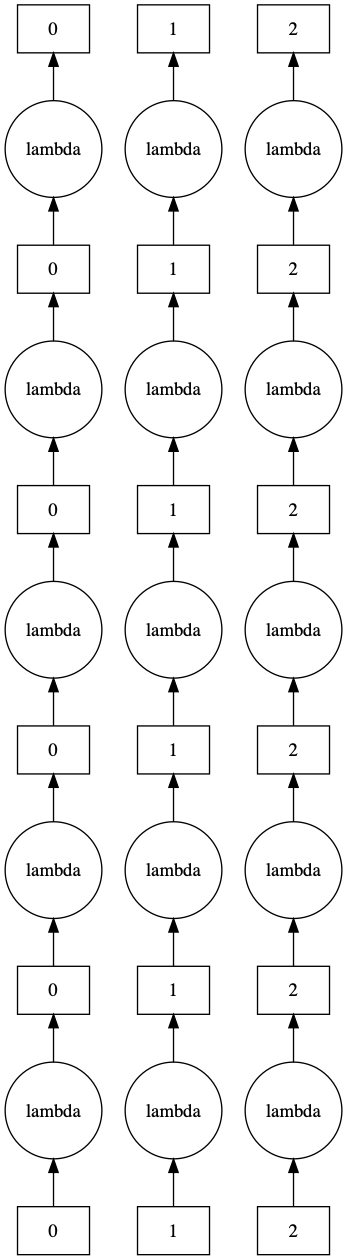
\includegraphics[width=0.125\textwidth,
    angle=-90]{images/incrementation-task-graph.png}
    \caption{Task graph for Incrementation with 5 iterations and 3 BigBrain blocks.
    Circles represent the incrementation and sleep function while rectangles
    represent stages of the image blocks.}\label{fig:tg-inc}
\end{figure}

\subsubsection{Histogram}

 Our second application calculates the histogram of the BigBrain image (see
 Algorithm~\ref{alg:histogram}). It reads the image blocks from the shared file
 system, calculates intensity frequencies, aggregates the frequencies across the
 blocks, and finally writes the resulting histogram to the shared file system as a
 single \SI{766}{\kilo\byte} file. This application implements a typical map-reduce
 pattern, where the final result is obtained from all the input blocks (see
 Fig.~\ref{fig:tg-histo}). This application requires data shuffling thus inter-worker
 communication. The total amount of shuffled data is however limited to
 \SI{2.62}{\mega\byte} per blocks as it only consists of image histograms.

\begin{algorithm}[!t]
    \caption{Histogram}\label{alg:histogram}
    \begin{algorithmic}
    \Require{\(files\), files containing BigBrain}
    \Require{\(fs\), NFS to save image to.}
    \ForEach{\(file \in files\)}
        \State{Read \(block\) from \(file\)}
        \State{{Calculate \(frequency\) of \(blocks\)}}
    \EndFor
    
    \State{\(histogram\gets\)Aggregate \(frequency\) of each \(file\)}

    \State{Write \(histogram\) to \(fs\)}
    \end{algorithmic}
\end{algorithm}

\begin{figure}[!t]
    \centering
    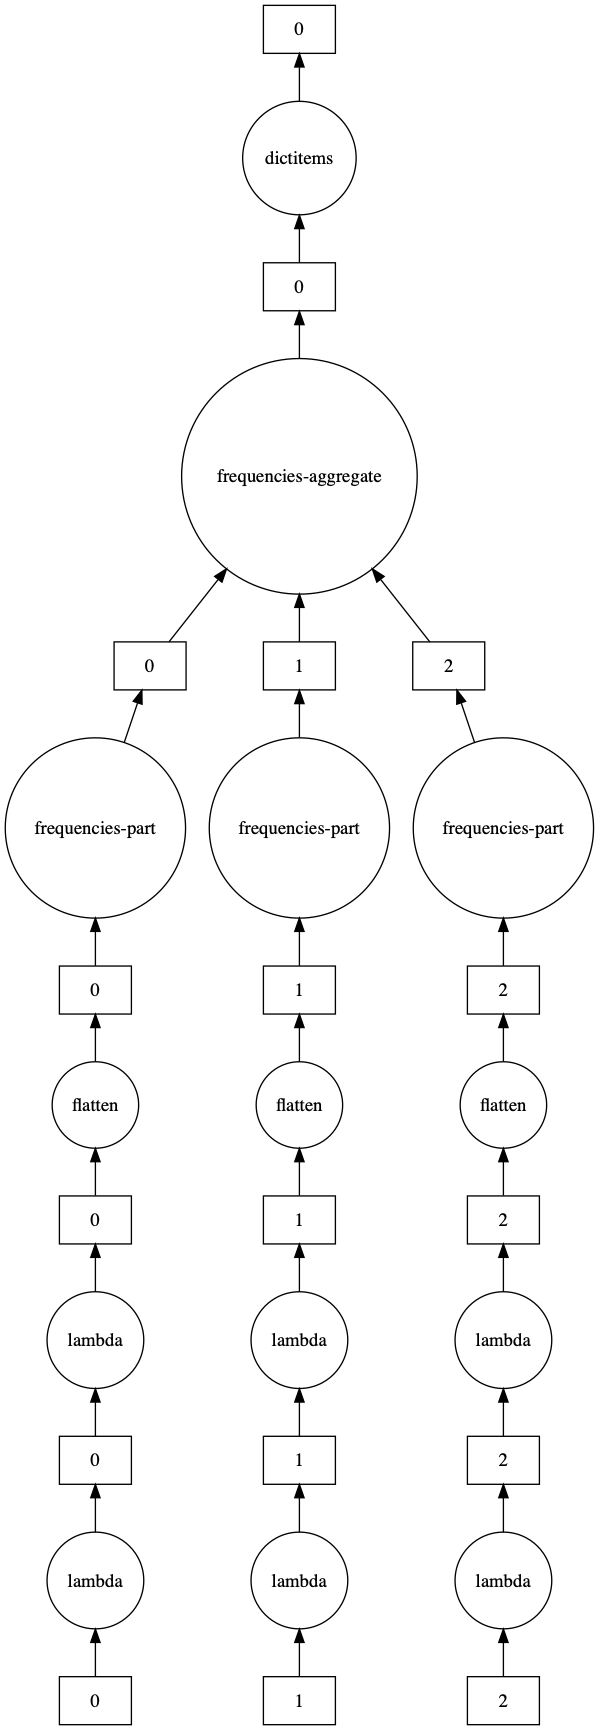
\includegraphics[width=0.16\textwidth, angle=-90]{images/histogram-task-graph.png}
    \caption{Task graph for Histogram with 3 BigBrain blocks. Circles represent the
    functions while rectangles represent stages of the image blocks.
    }\label{fig:tg-histo}
\end{figure}

\subsubsection{BIDS app example}

We used the \href{https://github.com/BIDS-Apps/example}{BIDS app example} application
available on GitHub. This application operates in a map-reduce way. The map phase,
also called participant analysis, extracts the brain tissues of a subject's 3D MRI
using the popular FMRIB Software Library
(\href{https://fsl.fmrib.ox.ac.uk/fsl/fslwiki}{FSL}), and writes the resulting image
(\SI{2.47}{\mega\byte} on average) to the shared file system. The reduce phase, also
called group analysis, computes the volume of each brain and returns the average
volume, shuffling a total of \SI{8.6}{\giga\byte} image data.

While Incrementation and Histogram were implemented directly in Python,
BIDS app example requires an external library and is distributed as a
Docker container image (bids/base\_fsl on DockerHub). To avoid remote file
transfers from DockerHub, we preloaded our OpenStack instances with the
Docker image, and started the Docker engine at startup.
\subsection{Experiments}

We varied four parameters in our experiments, as shown in
Table~\ref{tab:param}. We varied (1) the number of workers to assess the
scalability of the engines, (2) the number of BigBrain blocks in
Incrementation and Histogram to measure the effect of different IO patterns
and parallelization degrees, and (3) the number of iterations and sleep
delay in Incrementation to evaluate the effect of job length.
It should be noted that increasing the number of blocks or iterations also
increases the total compute time of the application for a given sleep
delay. To avoid any potential external bias such as background load on the
network, we ran the experiments in a randomized order and cleared the page
cache of each worker before each execution.

For each run, we measured the application makespan as well as the cumulative 
data read, compute, data write, and engine overhead across all application tasks. 
We measured the overhead by \TG{\ldots, maybe add a figure}.

\TG{explain that number of iterations may impact futures.}

% The baseline for our experiments is: 8 workers, 125 blocks, 10 iterations and 4
% seconds sleep delay.

\begin{table}[!t]
    \renewcommand{\arraystretch}{1.3}
    \caption{Parameters for the experiments}\label{tab:param}
    \centering
    \begin{tabular*}{\columnwidth}{llll}
    \hline
                        & Incrementation & Histogram             & BIDS Example          \\ \hline
    \# of worker        & 1, 2, 4, 8     & 1, 2, 4, 8            & 1, 2, 4, 8            \\
    \# of blocks        & 30, 125, 750   & 30, 125, 750          & 30, 125, 750          \\
    \# of iterations    & 1, 10, 100     & \multicolumn{1}{c}{-} & \multicolumn{1}{c}{-} \\
    Sleep delay {[}\SI{}{\second}{]} & 1, 4, 16, 64   & \multicolumn{1}{c}{-} & \multicolumn{1}{c}{-} \\ \hline
    \end{tabular*}
    \end{table}






%%%%% RESULTS %%%%%
\section{Results}

%%% INCREMENTATION %%%
%% worker
\subsection{Incrementation: Number of workers}
Figure~\ref{fig:inc_ms_worker} shows the makespan of the Incrementation application
for different numbers of workers and for different engines. The bars show the average
makespan over 5 repetitions while the error bars are the standard deviation. Overall,
there is no substantial makespan difference between the engines. Dask seems to have a
slight advantage over Spark, \SI{83.61}{\second} on average,
with Delayed and Futures being slightly better than Bags.

For all engines, the makespan is far from decreasing linearly with the
number of workers. Note that there are 8 threads per worker. The makespan
even increases between 4 and 8 workers. This is due to the high impact of
data transfers and engine overhead on the application. 

Figure~\ref{fig:inc_tt_worker} shows the total execution time of the
Incrementation application, broken down into data transfer (read and
write), compute (sleep), and overhead time. As expected, the computing time
stays similar when the number of workers increases. However, the data
transfer time and overhead increase proportionally to the number of
workers \TG{check if indeed proprotional, add regression slopes}.

On Figure~\ref{fig:inc_tt_worker}, we also note that Spark's overhead is
slightly lower than Dask's in particular as the number of workers increase.
Within Dask, Delayed and Futures have a higher overhead than Bags. However,
overhead differences are compensated by an increase of data transfer time,
as a reduced overhead increases the concurrency between data transfers. 

\begin{figure}[!b]
    \centering
    \begin{subfigure}[b]{\columnwidth}
        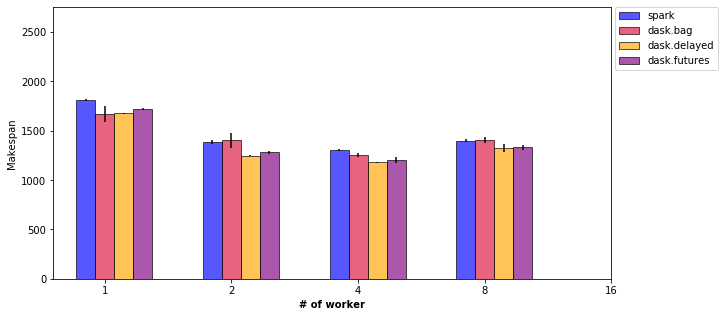
\includegraphics[clip,width=\columnwidth]{images/inc_worker.png}%
        \caption{Incrementation makespan}\label{fig:inc_ms_worker}
    \end{subfigure}
    \\
    \begin{subfigure}[b]{\columnwidth}
        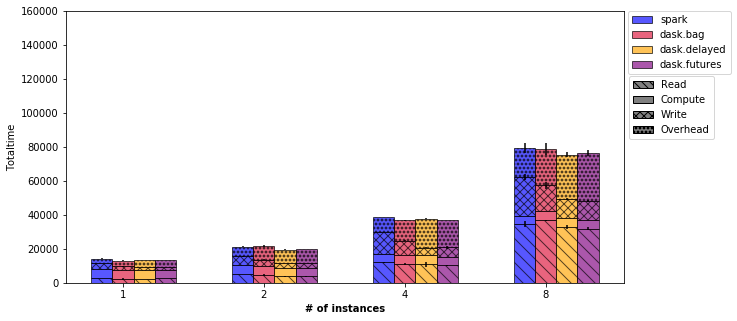
\includegraphics[clip,width=\columnwidth]{images/inc_idle_worker.png}%
        \caption{Incrementation total time}\label{fig:inc_tt_worker}
    \end{subfigure}
    \caption{125 blocks, 10 iterations, \SI{4}{\second} delay, 8 threads/worker}\label{fig:inc_worker}
\end{figure}

% blocks
\subsection{Incrementation: Number of blocks}

Figure~\ref{fig:inc_ms_block} shows the Incrementation makespan when varying the
number of image blocks for a constant BigBrain image size. We were not able to run
Spark for 30 blocks due to its \SI{2}{\giga\byte} limitation in the task size it can
compute. Once again, we do not observe any significant difference among the engines.
For all engines, makespan variability increases with the number of blocks, however,
engines scale very well in general.


In Figure~\ref{fig:inc_tt_block}, the total execution time of each function is shown.
For 30 blocks the Dask Bag API has a much lower overhead time. This is because Dask
Bag was only using one thread per block in comparison to Dask Delayed and Dask
Futures which were offloading a block calculations on multiple threads of the same
worker. Once again, the data transfer time reduces with more blocks however the
overhead time increases by a similar amount. This is not observed for 30 blocks as
the workers are not used at full capacity, i.e., some threads are idle. Finally, the
variability of the overhead increases with the number of blocks, which explains the
makespan variability mentioned previously.

\begin{figure}[!t]
    \centering
    \begin{subfigure}[b]{\columnwidth}
        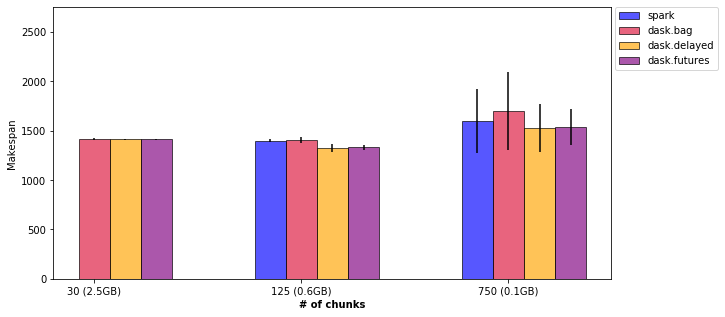
\includegraphics[clip,width=\columnwidth]{images/inc_block.png}%
        \caption{Incrementation makespan}\label{fig:inc_ms_block}
    \end{subfigure}
    \\
    \begin{subfigure}[b]{\columnwidth}
        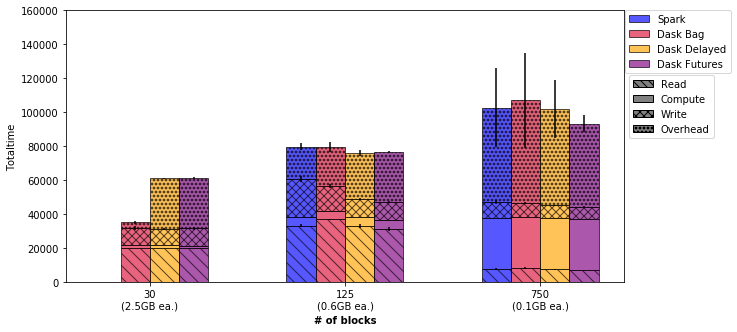
\includegraphics[clip,width=\columnwidth]{images/inc_idle_block.png}%
        \caption{Incrementation total time}\label{fig:inc_tt_block}
    \end{subfigure}
    \caption{10 iterations, \SI{4}{\second} delay, 8 workers, 8 threads/worker}\label{fig:inc_block}
\end{figure}

%% Iterations
\subsection{Incrementation: Number of iterations}
Figure~\ref{fig:inc_ms_itr} shows the makespan of the application while
varying the number of iterations. Overall,  Spark and Dask APIs are once
again equivalent, although Dask Delayed and Futures are slightly faster
than Bags and Spark for 1 and 10 few iterations, and Fuures are faster than
Delayed, Bags and Spark for 100 iterations. Differences remain minor
though.

In Figure~\ref{fig:inc_tt_itr}, the total execution time breakdown is
shown. We observe good scalability of all the engines with the number of
iterations.

% We think this is because Dask Delayed often
% schedule a block on a different thread of the same worker which causes small delays
% every time due to inter-thread data communication. This is good when there are fewer
% tasks as is make the IO between blocks go out of sync hence lowering the IO
% bottleneck however as the number of tasks increases those small delays become
% significant.

%  The Dask Futures API seems to outperform all the other APIs but this is
% most likely because the tasks are not interdependent thus this application benefits
% from the less optimal but faster scheduling brought by Dask Futures.

\begin{figure}[!t]
    \centering
    \begin{subfigure}[b]{\columnwidth}
        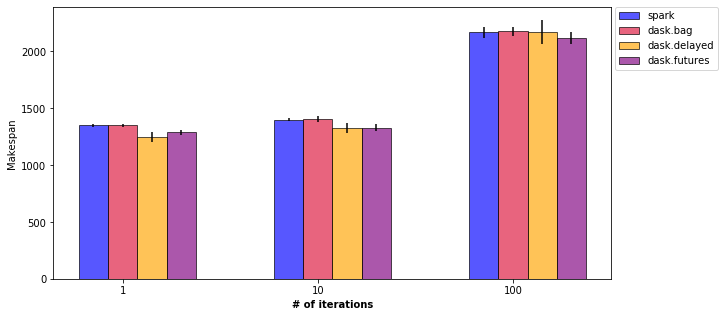
\includegraphics[clip,width=\columnwidth]{images/inc_itr.png}%
        \caption{Incrementation makespan}\label{fig:inc_ms_itr}
    \end{subfigure}
    \\
    \begin{subfigure}[b]{\columnwidth}
        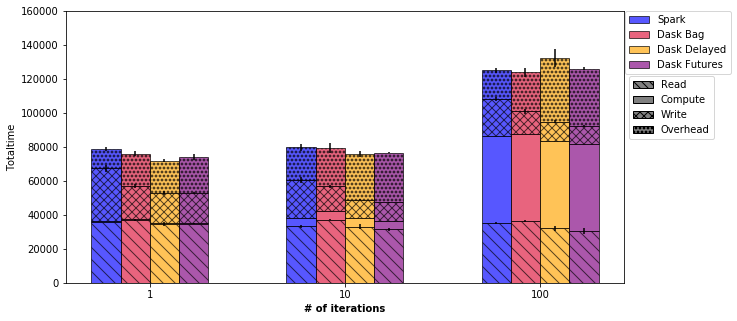
\includegraphics[clip,width=\columnwidth]{images/inc_idle_itr.png}%
        \caption{Incrementation total time}\label{fig:inc_tt_itr}
    \end{subfigure}
    \caption{125 blocks, \SI{4}{\second} delay, 8 workers, 8 threads/worker}
\end{figure}

%% Sleep time
\subsection{Incrementation: Sleep delay}
Figure~\ref{fig:inc_ms_sleep} shows the makespan of the Incrementation
application for different sleep delays. Overall, all engines again perform the same, and scale well with task duration.
 Spark is initially slower than the
Dask APIs, however, it is faster when increasing the sleep delay. Also,
within the Dask APIs, Dask Bag is slower than the other two but it is not
considerable.

Figure~\ref{fig:inc_tt_sleep} shows the total execution time breakdown. On
one hand, Spark has the smallest overhead. As previously observed,
variations in overhead time are almost exactly compensated by variations in data
transfer time.

% \begin{table}[!t]
%     \caption{Function time for the sleep experiment}
%     \begin{subtable}[b]{\columnwidth}
%         \renewcommand{\arraystretch}{1.3}
%         \caption{Overhead time in second}\label{tab:inc_sleep_overhead}
%         \centering
%         \begin{tabular}{lllll}
%         \hline
%                      & 1 sec. & 4 sec. & 16 sec. & 64 sec. \\ \hline
%         Spark        & 14992  & 17076  & 16069   & 9769    \\
%         Dask.Bag     & 20690  & 21388  & 17759   & 18720   \\
%         Dask.Delayed & 27481  & 26199  & 22080   & 24624   \\
%         Dask.Futures & 27069  & 27984  & 23538   & 24762   \\ \hline
%         \end{tabular}
%     \end{subtable}
%     \vskip 0.2cm
%     \begin{subtable}[b]{\columnwidth}
%         \renewcommand{\arraystretch}{1.3}
%         \caption{IO time in second}\label{tab:inc_sleep_io}
%         \centering
%         \begin{tabular}{lllll}
%         \hline
%                      & 1 sec. & 4 sec. & 16 sec. & 64 sec. \\ \hline
%         Spark        & 63622  & 57144  & 51070   & 57078   \\
%         Dask.Bag     & 54630  & 52312  & 53743   & 53612   \\
%         Dask.Delayed & 45239  & 44142  & 45133   & 46198   \\
%         Dask.Futures & 46537  & 43161  & 44749   & 45846   \\ \hline
%         \end{tabular}
%     \end{subtable}
%     \vspace{-3mm}
%  \end{table}

\begin{figure}[!t]
    \centering
    \begin{subfigure}[b]{\columnwidth}
        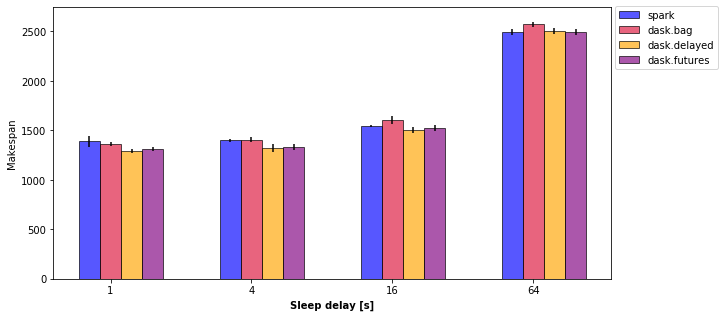
\includegraphics[clip,width=\columnwidth]{images/inc_sleep.png}%
        \caption{Incrementation makespan}\label{fig:inc_ms_sleep}
    \end{subfigure}
    \\
    \begin{subfigure}[b]{\columnwidth}
        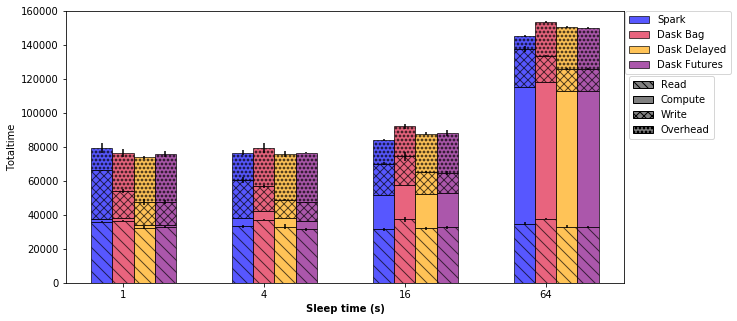
\includegraphics[clip,width=\columnwidth]{images/inc_idle_sleep.png}%
        \caption{Incrementation total time}\label{fig:inc_tt_sleep}
    \end{subfigure}
    \caption{125 blocks, 10 iterations, 8 workers, 8 threads/worker}
\end{figure}

%% Baseline gantt chart
\subsection{Incrementation: Gantt chart}

Figure~\ref{fig:inc_gantt} shows the Gantt chart obtained for each engine and API,
for a baseline execution with 125 blocks, a \SI{4}{\second} sleep delay and 8
workers. Gantt charts are structured in batches of up to 64 read-compute-write
concurrent sequences. File reads in the first batch are much longer than in the
following ones: this is due to the high synchronization of data transfers that leads
to a high saturation of the shared file system. We also note that overhead,
represented in white, is concentrated around the data transfer tasks \TG{find out
why}, and the computing tasks that run concurrently with data transfers. 
% The frameworks have similar makespan however the time spend for each type of
% task differs considerably (see Table~\ref{tab:inc_base}). Spark tends to spend more
% time than other frameworks for IO however it has a much lower overhead. Dask Delayed
% and Futures have the lowest IO time but a much higher overhead. Dask Bag stands in
% the middle for both IO and overhead. Compute time is approximately the same for all
% frameworks. Apart from the first IO section, there is a large amount of ovehead
% everytime time IO is performed. This is true for all frameworks.

\begin{figure*}[!htb]
    \centering
    \begin{subfigure}[b]{\columnwidth}
        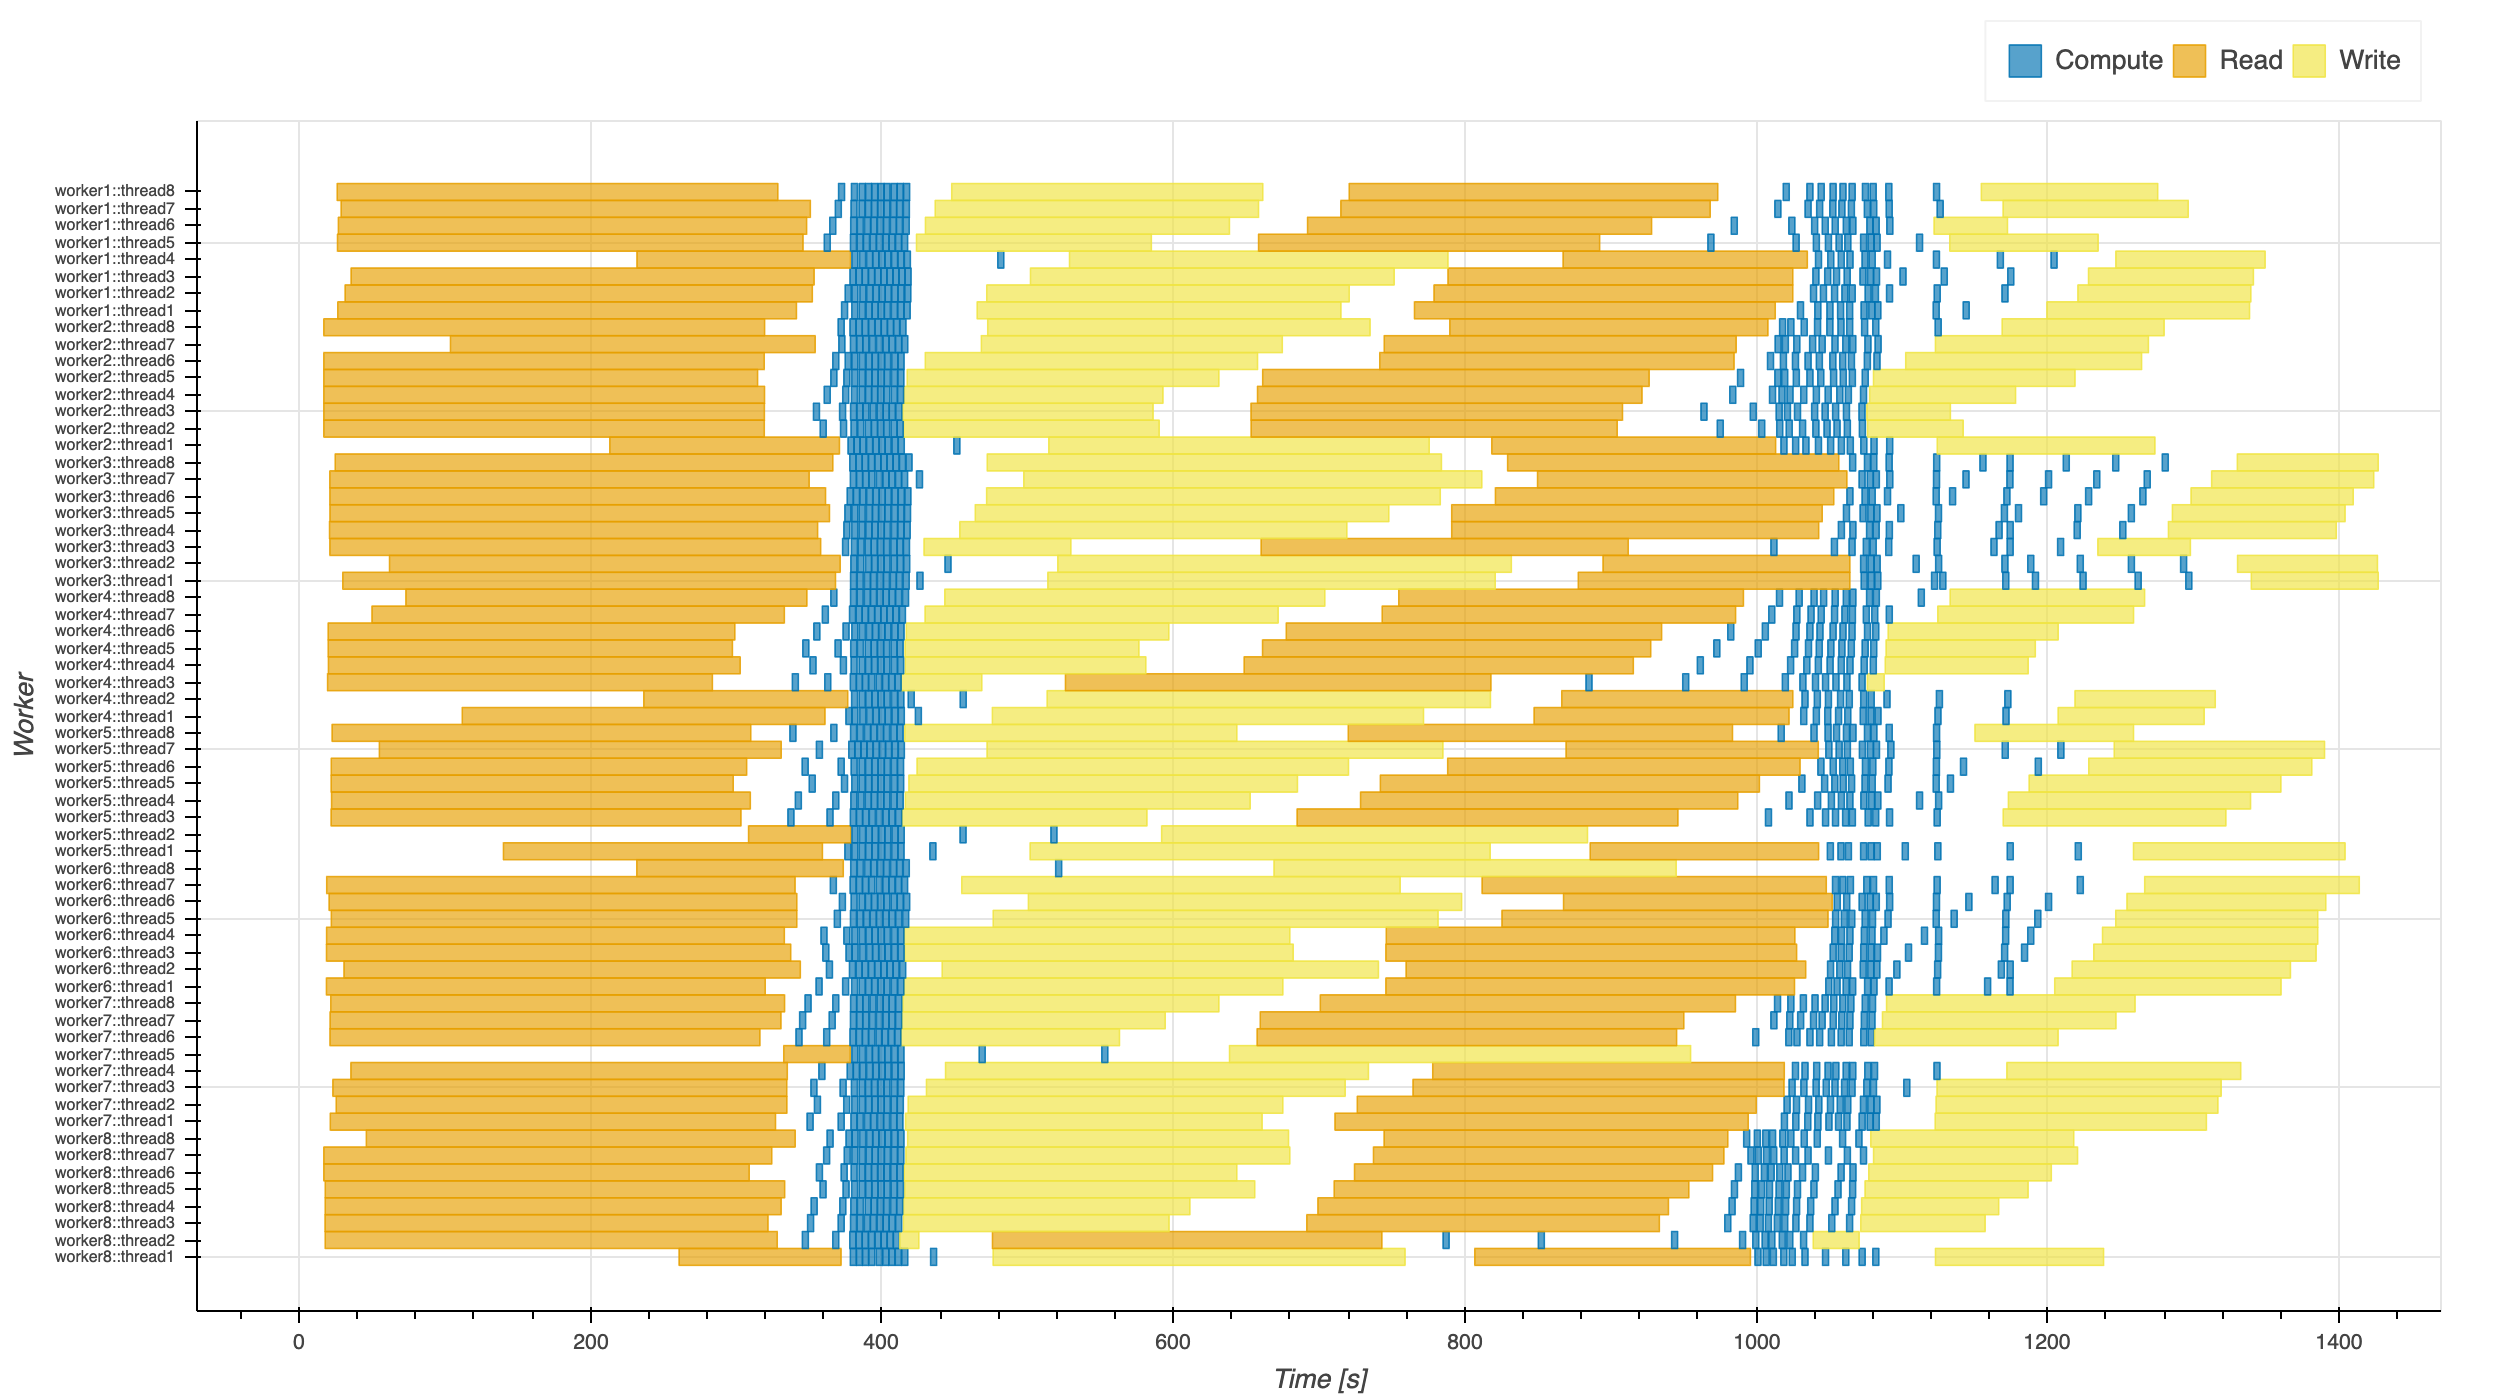
\includegraphics[clip,width=\columnwidth]{images/spark_inc_gantt.png}
        \caption{Spark}\label{fig:inc_spark_gantt}
    \end{subfigure}
    \hfill
    \begin{subfigure}[b]{\columnwidth}
        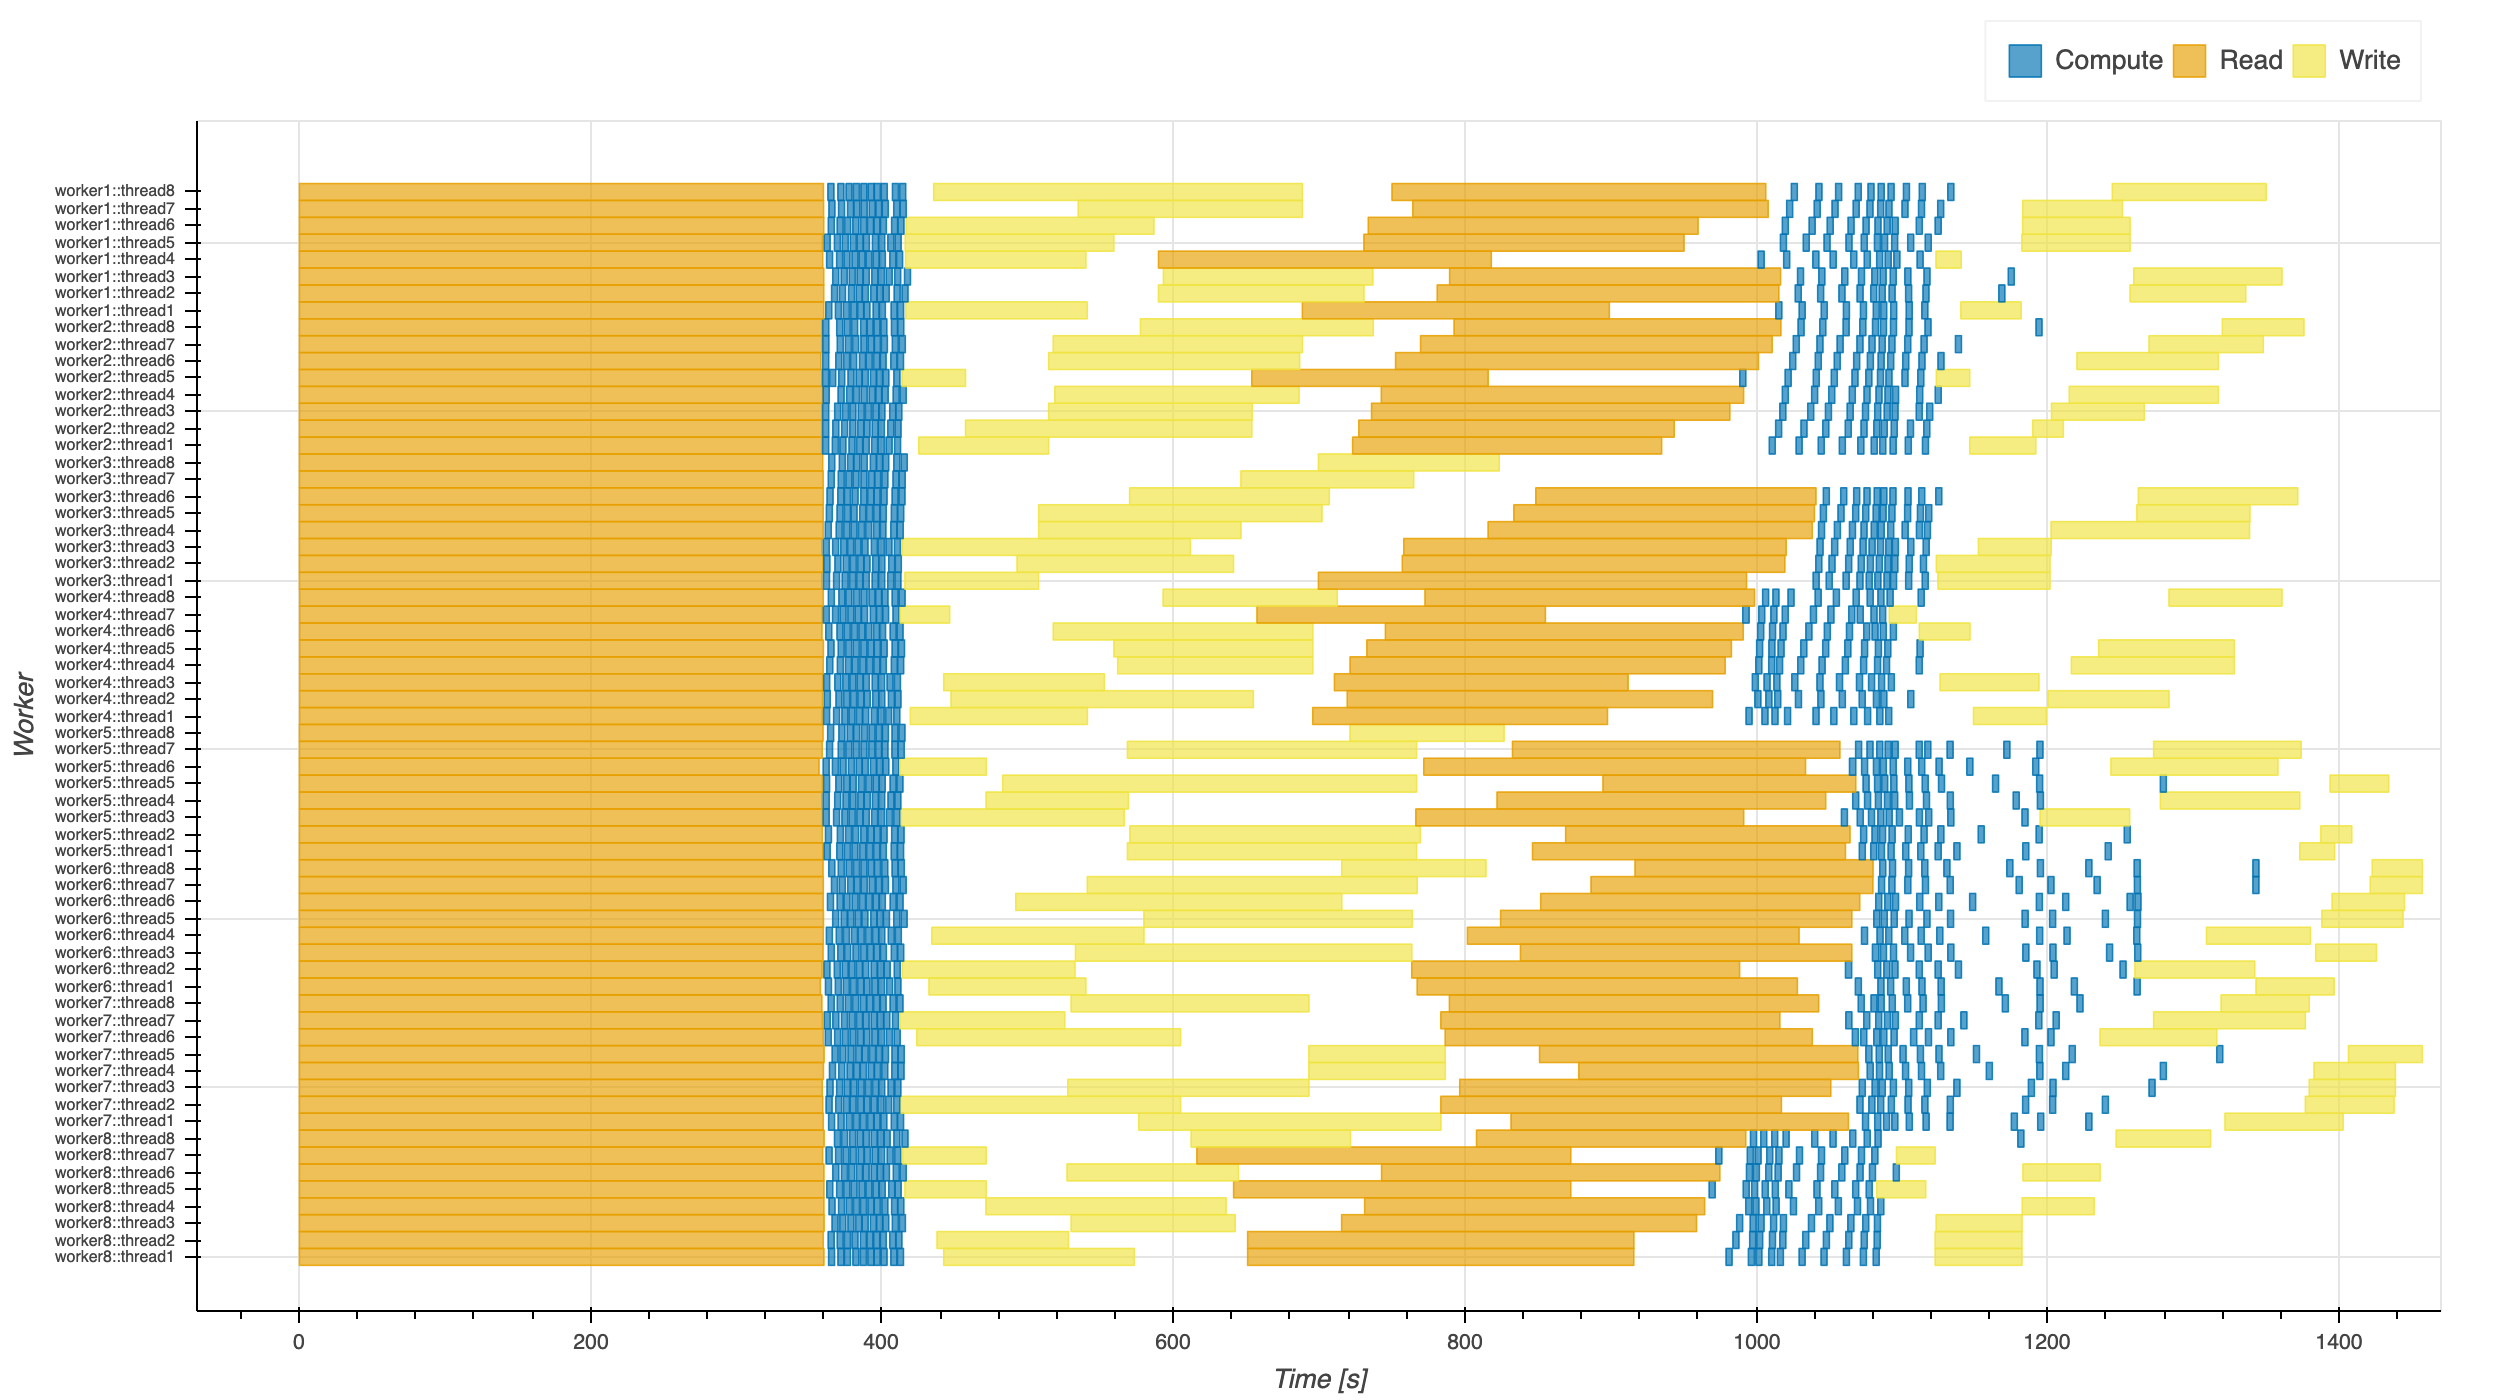
\includegraphics[clip,width=\columnwidth]{images/bag_inc_gantt.png}%
        \caption{Dask Bag}\label{fig:inc_dask_bag_gantt}
    \end{subfigure}
    \\
    \begin{subfigure}[b]{\columnwidth}
        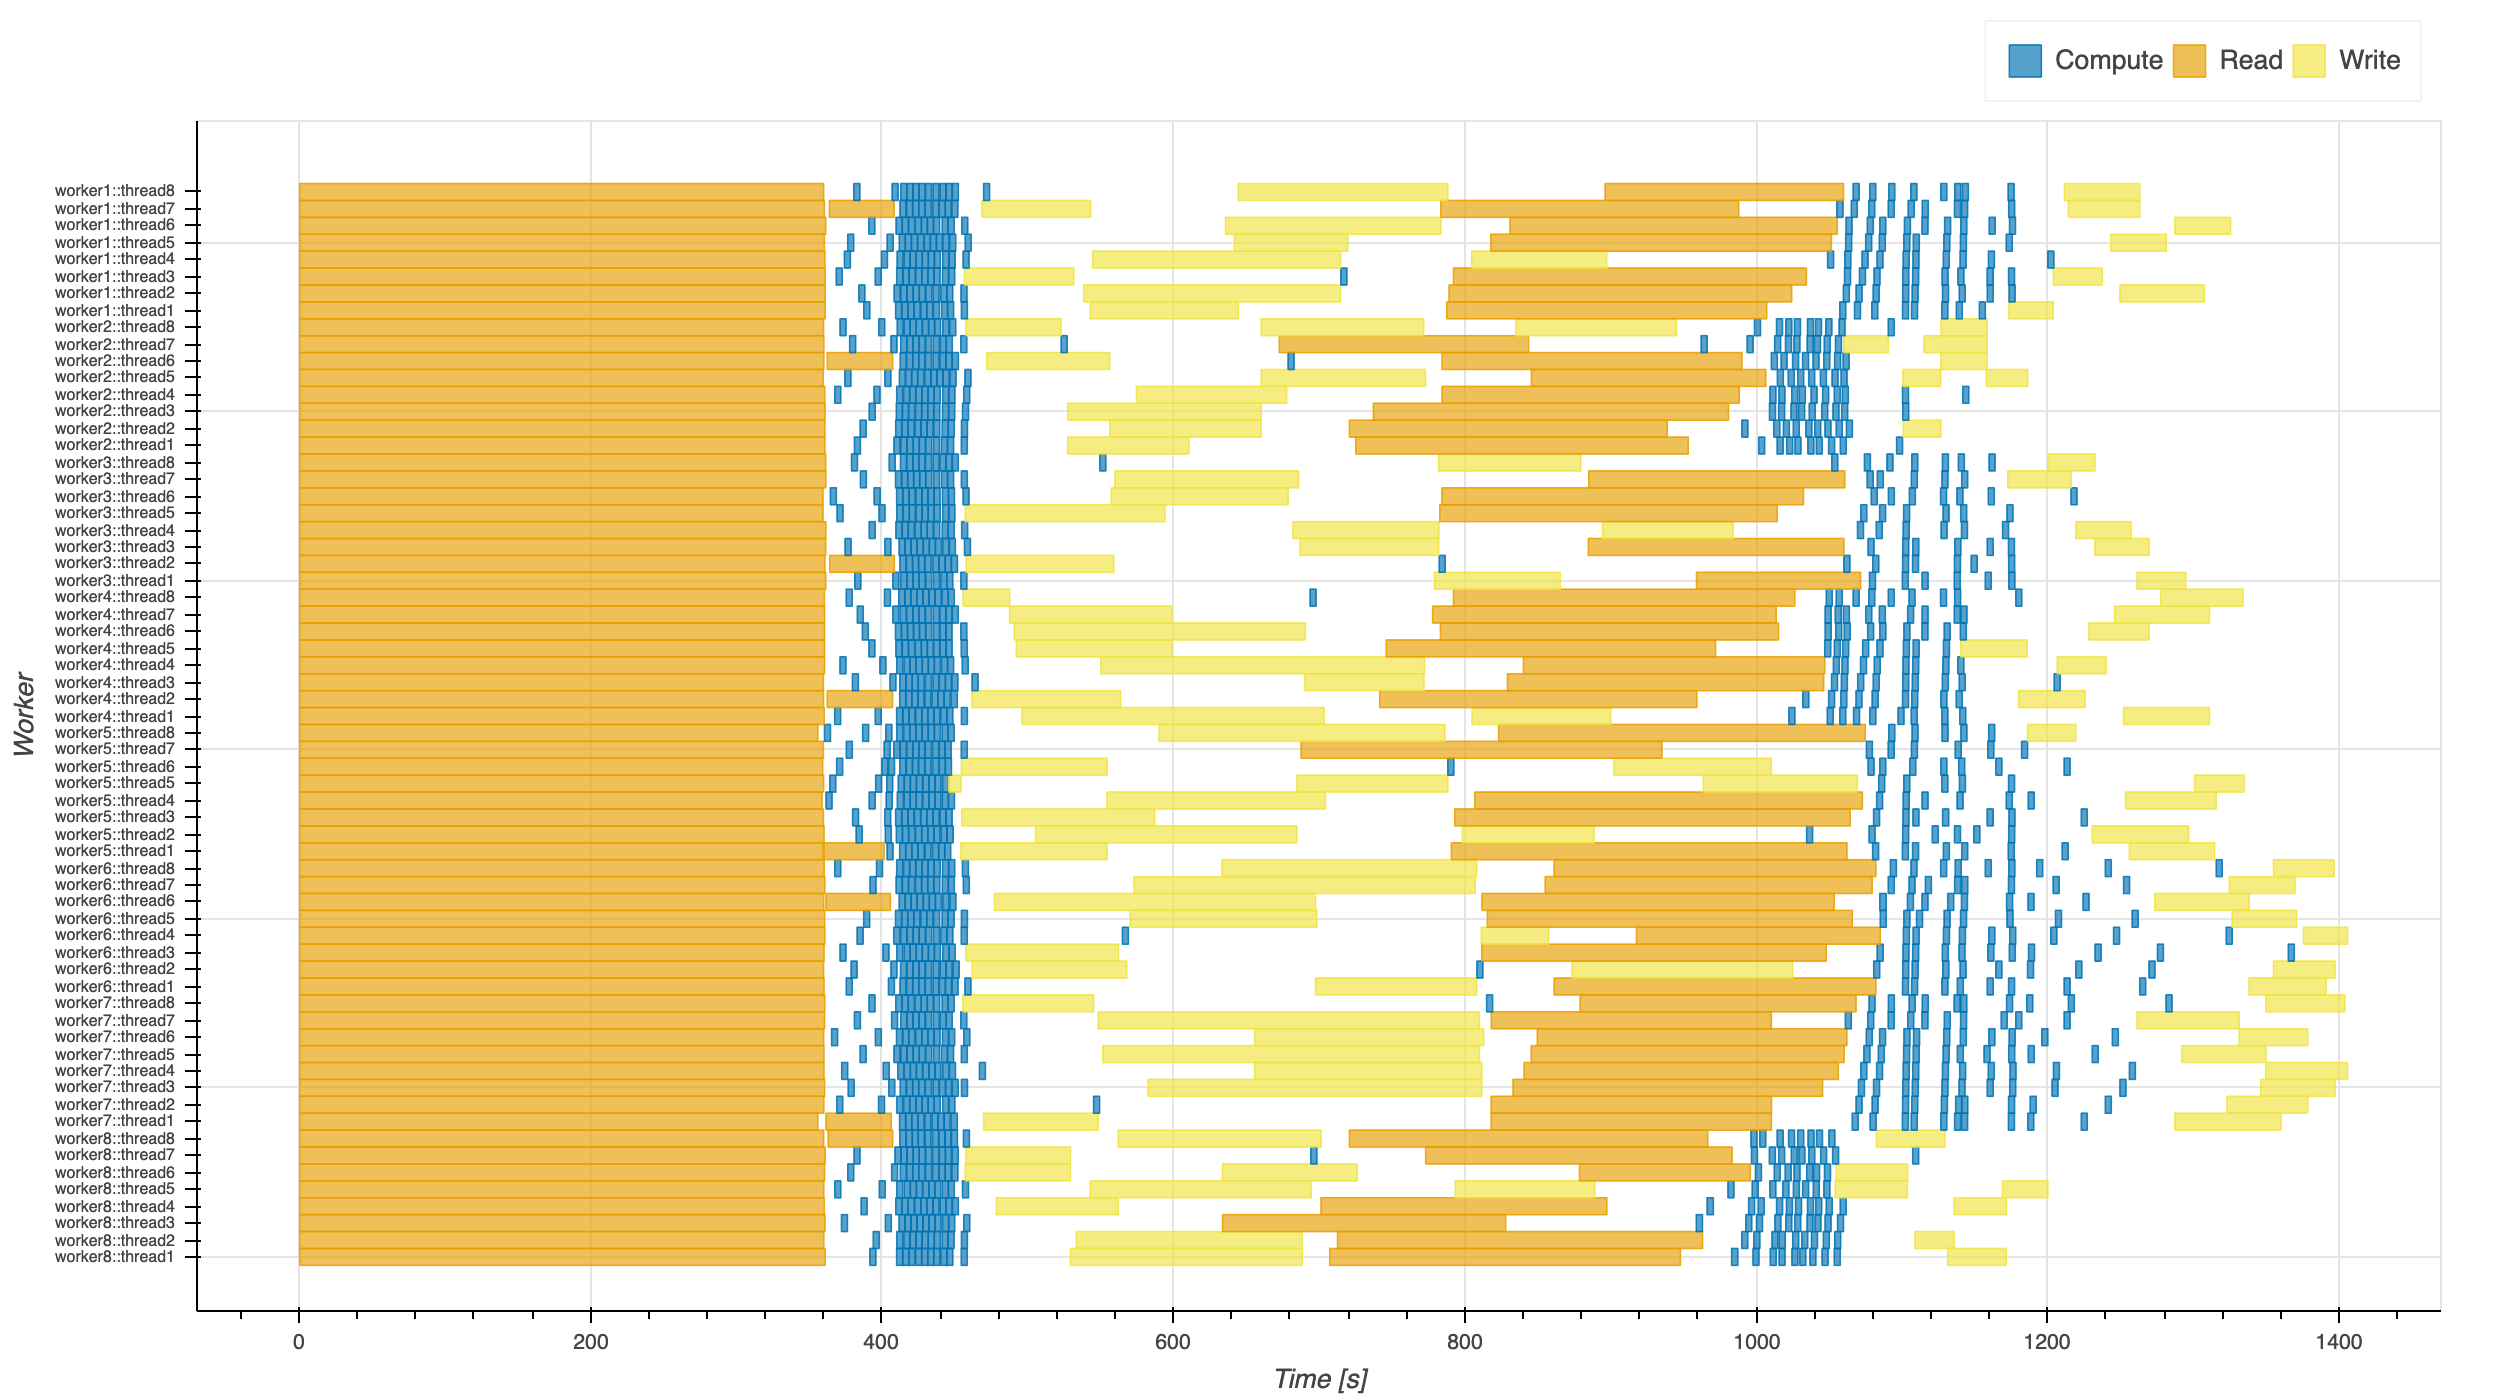
\includegraphics[clip,width=\columnwidth]{images/delayed_inc_gantt.png}%
        \caption{Dask Delayed}\label{fig:inc_dask_delayed_gantt}
    \end{subfigure}
    \hfill
    \begin{subfigure}[b]{\columnwidth}
        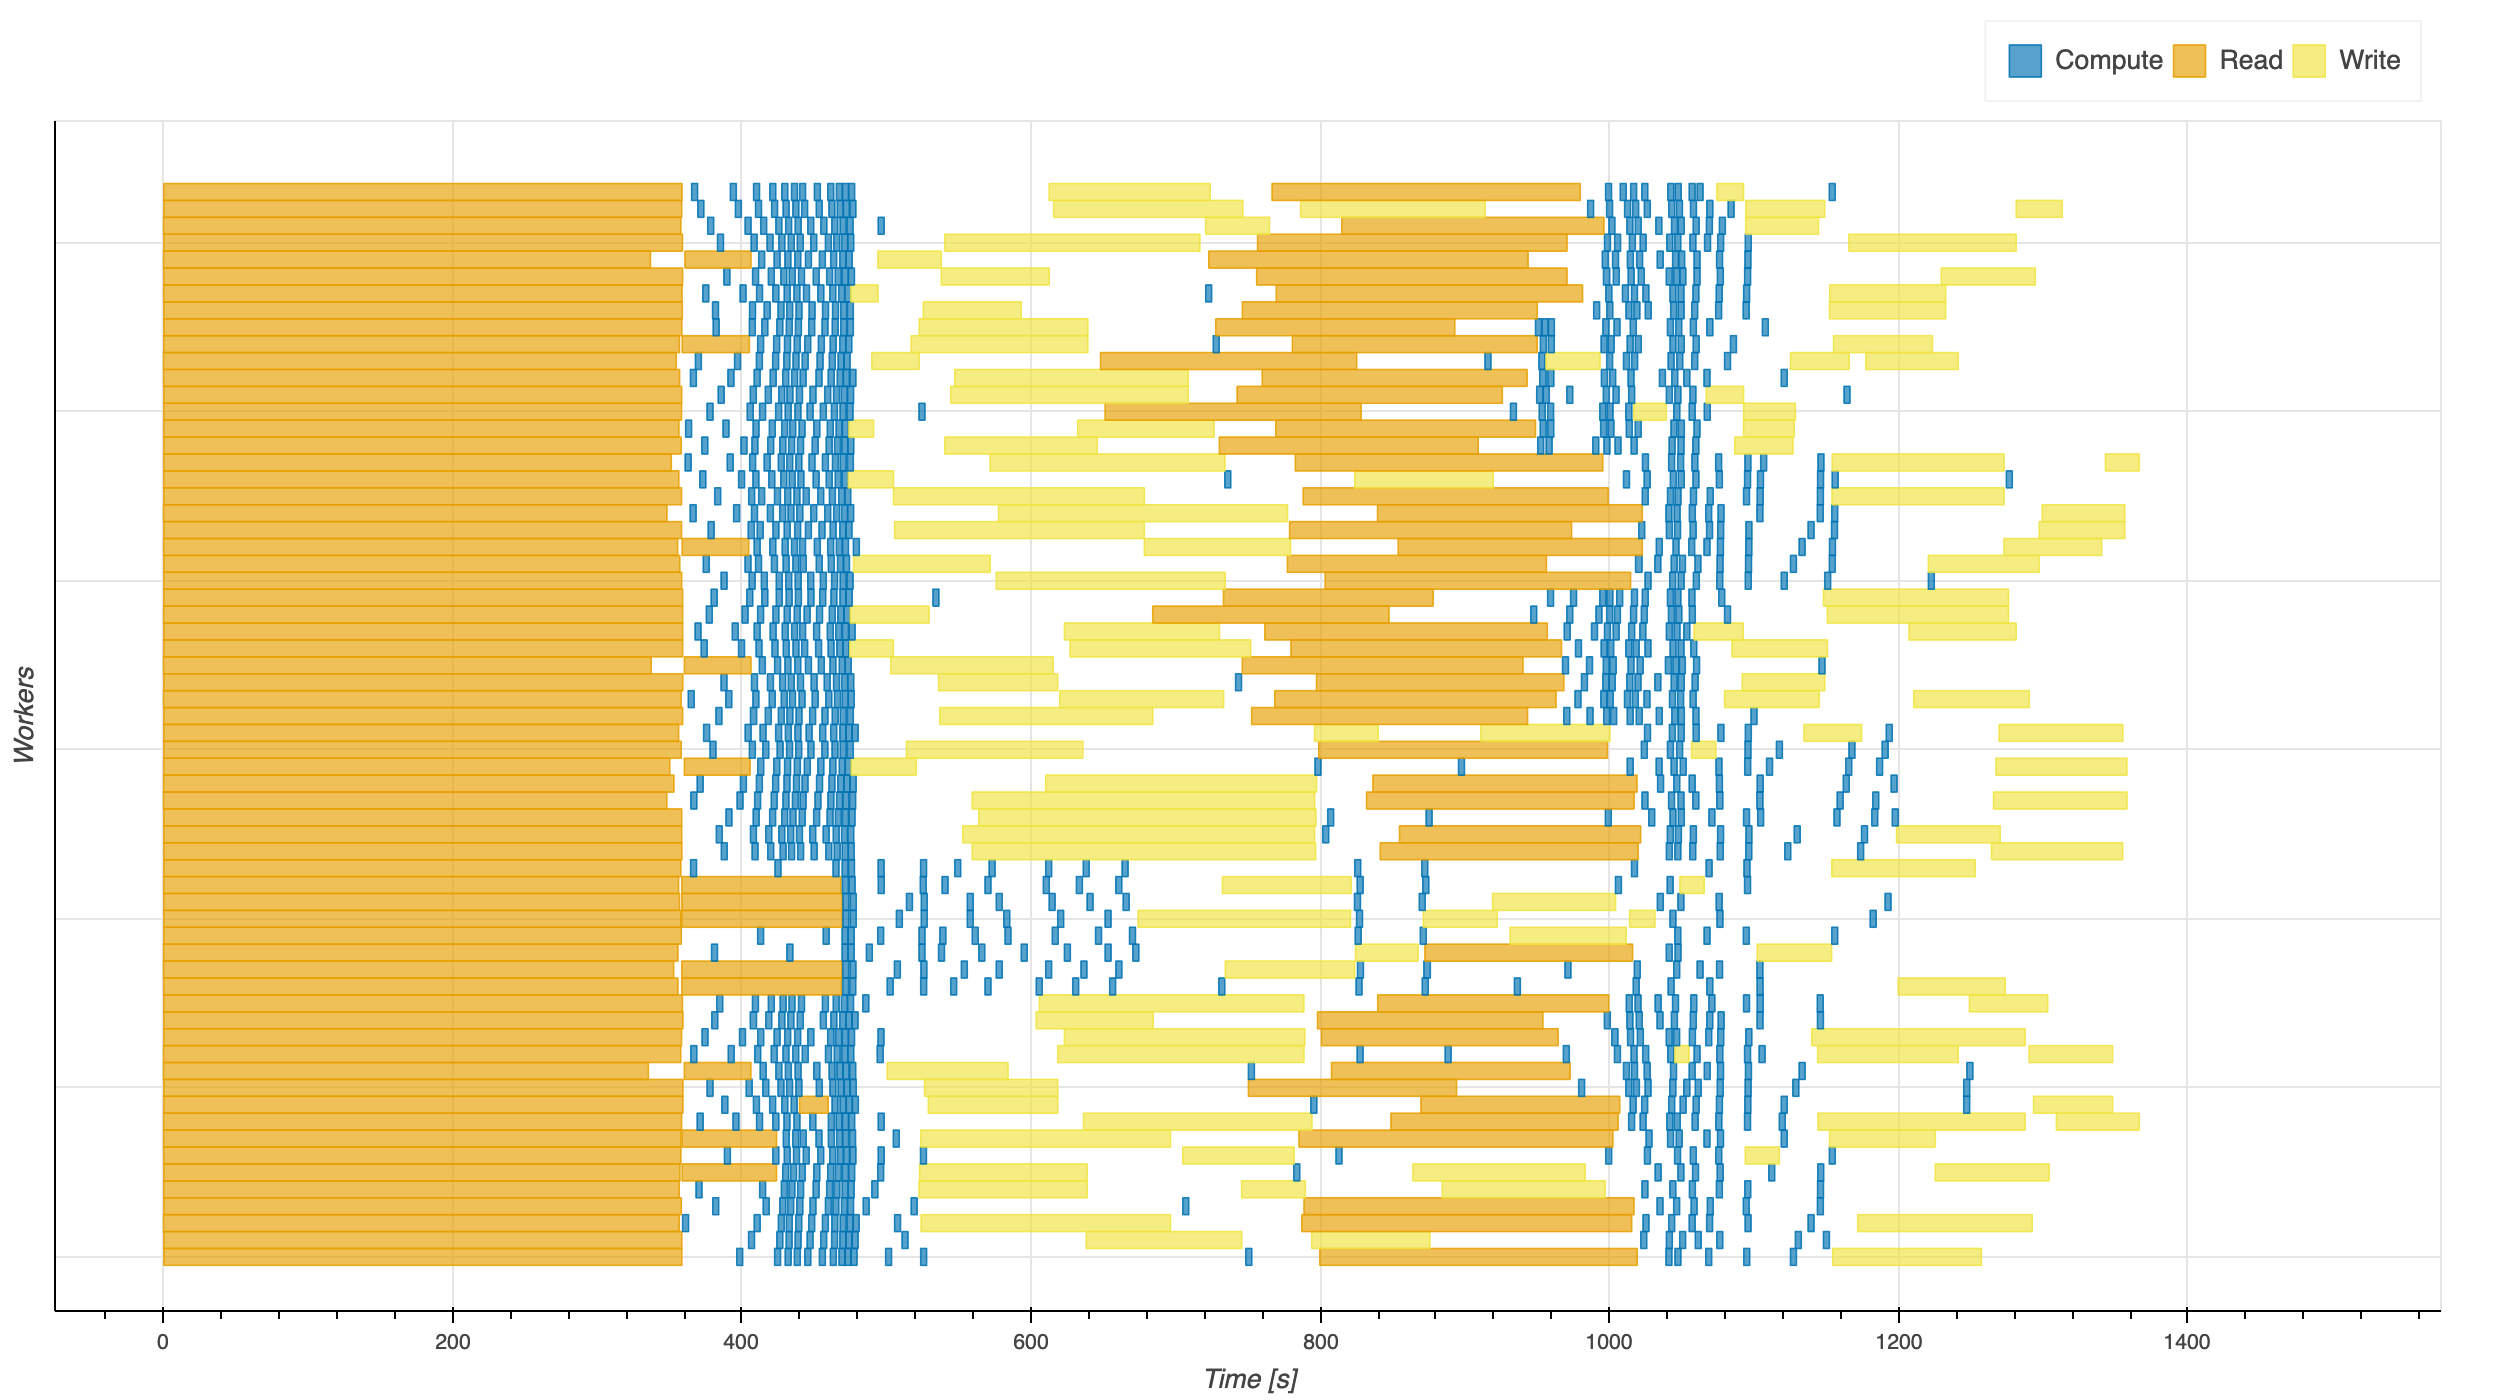
\includegraphics[clip,width=\columnwidth]{images/futures_inc_gantt.png}%
        \caption{Dask Futures}\label{fig:inc_dask_futures_gantt}
    \end{subfigure}
    \caption{Gantt chart with 125 blocks, \SI{4}{\second} delay, 8 workers}\label{fig:inc_gantt}
\end{figure*}

% \begin{table}[!b]
%     \renewcommand{\arraystretch}{1.3}
%     \caption{Distribution of the execution time in second: 125 blocks, 4 sec.\ sleep
%     delay, 10 iterations, and 8 workers}\label{tab:inc_base}
%     \centering
%     \begin{tabular*}{\columnwidth}{llllll}
%     \hline
%                  & Read  & Compute & Write & Overhead & Total \\ \hline
%     Spark        & 34465 & 5118    & 22679 & 17076    & 79338 \\
%     Dask Bag     & 36863 & 5121    & 15449 & 21388    & 78821 \\
%     Dask Delayed & 32769 & 5119    & 11373 & 26199    & 75461 \\
%     Dask Futures & 31891 & 5120    & 11270 & 27984    & 76265 \\ \hline
%     \end{tabular*}
%  \end{table}

%%% HISTOGRAM %%%
\subsection{Histogram: Number of workers}

\begin{figure}[!t]
    \centering
    \begin{subfigure}[b]{\columnwidth}
        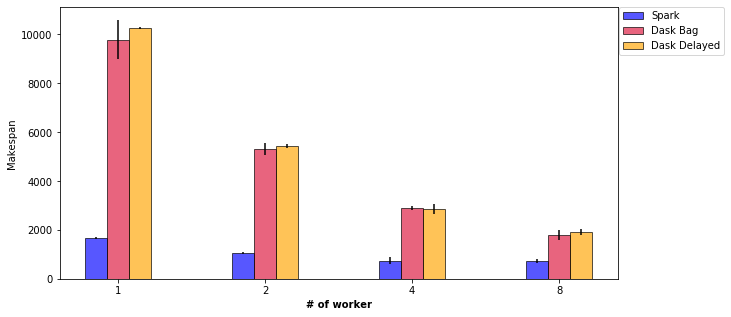
\includegraphics[clip,width=\columnwidth]{images/histo_worker.png}%
        \caption{Histogram makespan}\label{fig:histo_ms_worker}
    \end{subfigure}
    \\
    \begin{subfigure}[b]{\columnwidth}
        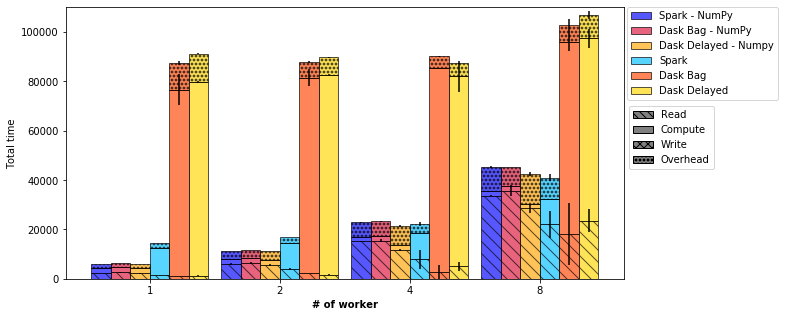
\includegraphics[clip,width=\columnwidth]{images/histo_idle_worker.png}%
        \caption{Histogram total time}\label{fig:histo_tt_worker}
    \end{subfigure}
    \caption{125 blocks}
\end{figure}

\subsection{Histogram: Number of blocks}

\begin{figure}[!t]
    \centering
    \begin{subfigure}[b]{\columnwidth}
        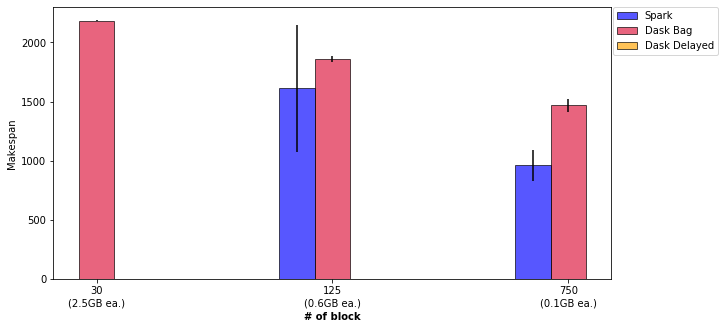
\includegraphics[clip,width=\columnwidth]{images/histo_block.png}%
        \caption{Histogram makespan}\label{fig:histo_ms_block}
    \end{subfigure}
    \\
    \begin{subfigure}[b]{\columnwidth}
        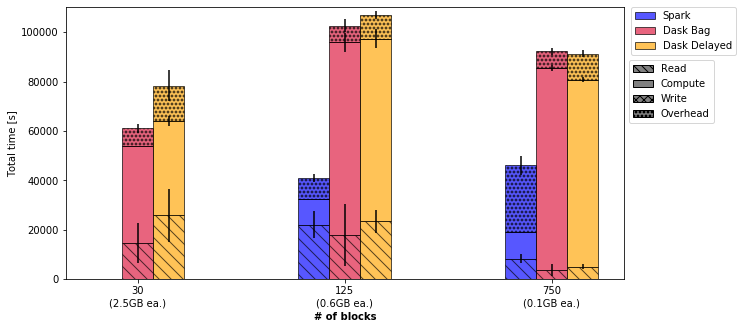
\includegraphics[clip,width=\columnwidth]{images/histo_idle_block.png}%
        \caption{Histogram total time}\label{fig:histo_tt_block}
    \end{subfigure}
    \caption{8 workers}
\end{figure}
\TG{We decided to omit Dask Futures as it does not have any value over Dask
Delayed in this application.}



%%% BIDS EXAMPLE %%%
\subsection{BidsApp example: Number of workers}

\begin{figure}[!t]
    \centering
    \begin{subfigure}[b]{\columnwidth}
        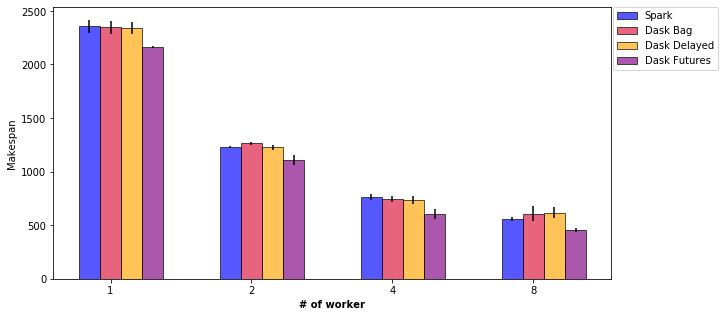
\includegraphics[clip,width=\columnwidth]{images/bids_worker.png}%
        \caption{Histogram makespan}\label{fig:bids_ms_worker}
    \end{subfigure}
    \\
    \begin{subfigure}[b]{\columnwidth}
        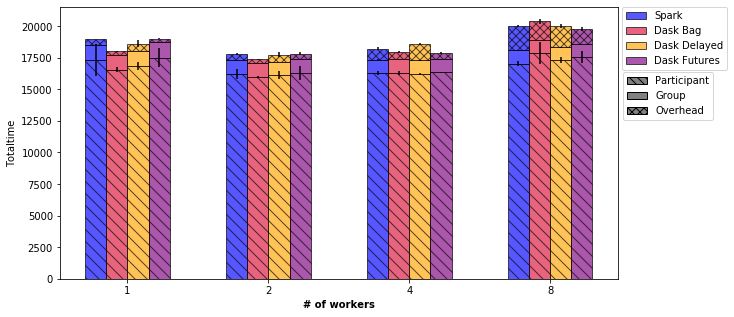
\includegraphics[clip,width=\columnwidth]{images/bids_idle_worker.png}%
        \caption{Histogram total time}\label{fig:bids_tt_worker}
    \end{subfigure}
    \caption{Variation of the amount of worker, 8 threads/worker}
\end{figure}


%% Baseline gantt chart
\subsection{BidsApp example: Gantt chart}

% Figure~\ref{fig:inc_gantt} shows the Gantt chart obtained for each engine and API,
% for a baseline execution with 125 blocks, a \SI{4}{\second} sleep delay and 8
% workers. Gantt charts are structured in batches of up to 64 read-compute-write
% concurrent sequences. File reads in the first batch are much longer than in the
% following ones: this is due to the high synchronization of data transfers that leads
% to a high saturation of the shared file system. We also note that overhead,
% represented in white, is concentrated around the data transfer tasks \TG{find out
% why}, and the computing tasks that run concurrently with data transfers. 
% The frameworks have similar makespan however the time spend for each type of
% task differs considerably (see Table~\ref{tab:inc_base}). Spark tends to spend more
% time than other frameworks for IO however it has a much lower overhead. Dask Delayed
% and Futures have the lowest IO time but a much higher overhead. Dask Bag stands in
% the middle for both IO and overhead. Compute time is approximately the same for all
% frameworks. Apart from the first IO section, there is a large amount of ovehead
% everytime time IO is performed. This is true for all frameworks.

\begin{figure*}[!htb]
    \centering
    \begin{subfigure}[b]{\columnwidth}
        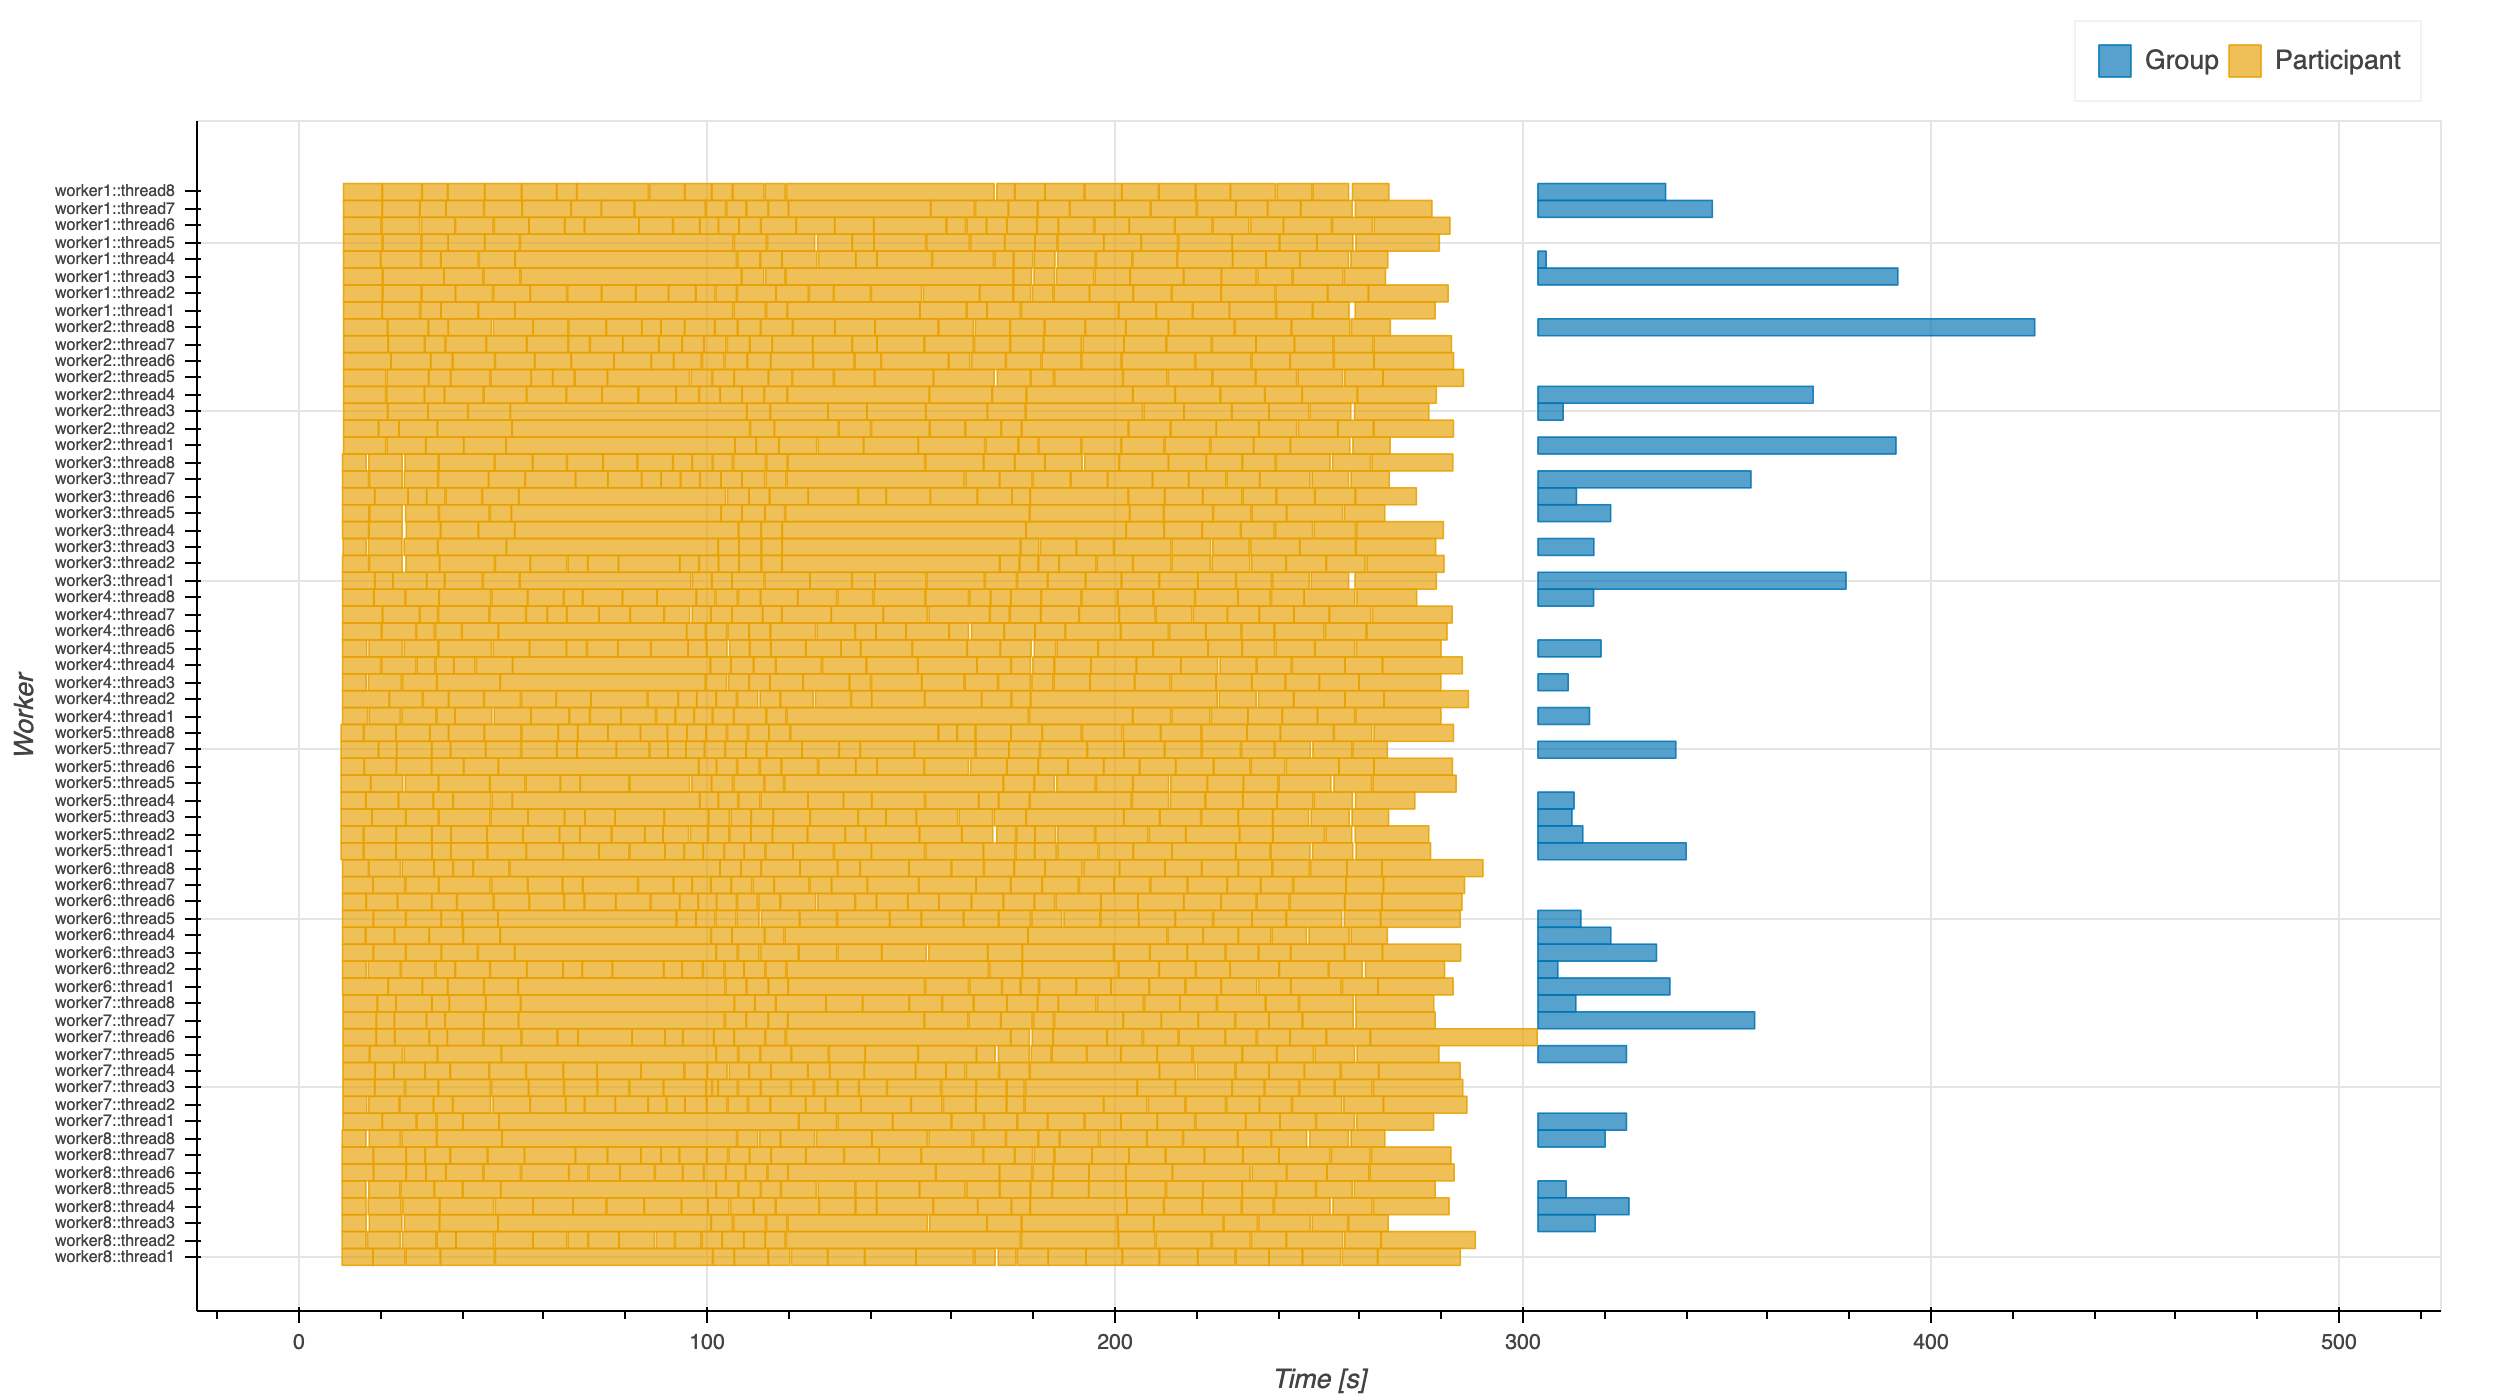
\includegraphics[clip,width=\columnwidth]{images/spark_bids_gantt.png}
        \caption{Spark}\label{fig:bids_spark_gantt}
    \end{subfigure}
    \hfill
    \begin{subfigure}[b]{\columnwidth}
        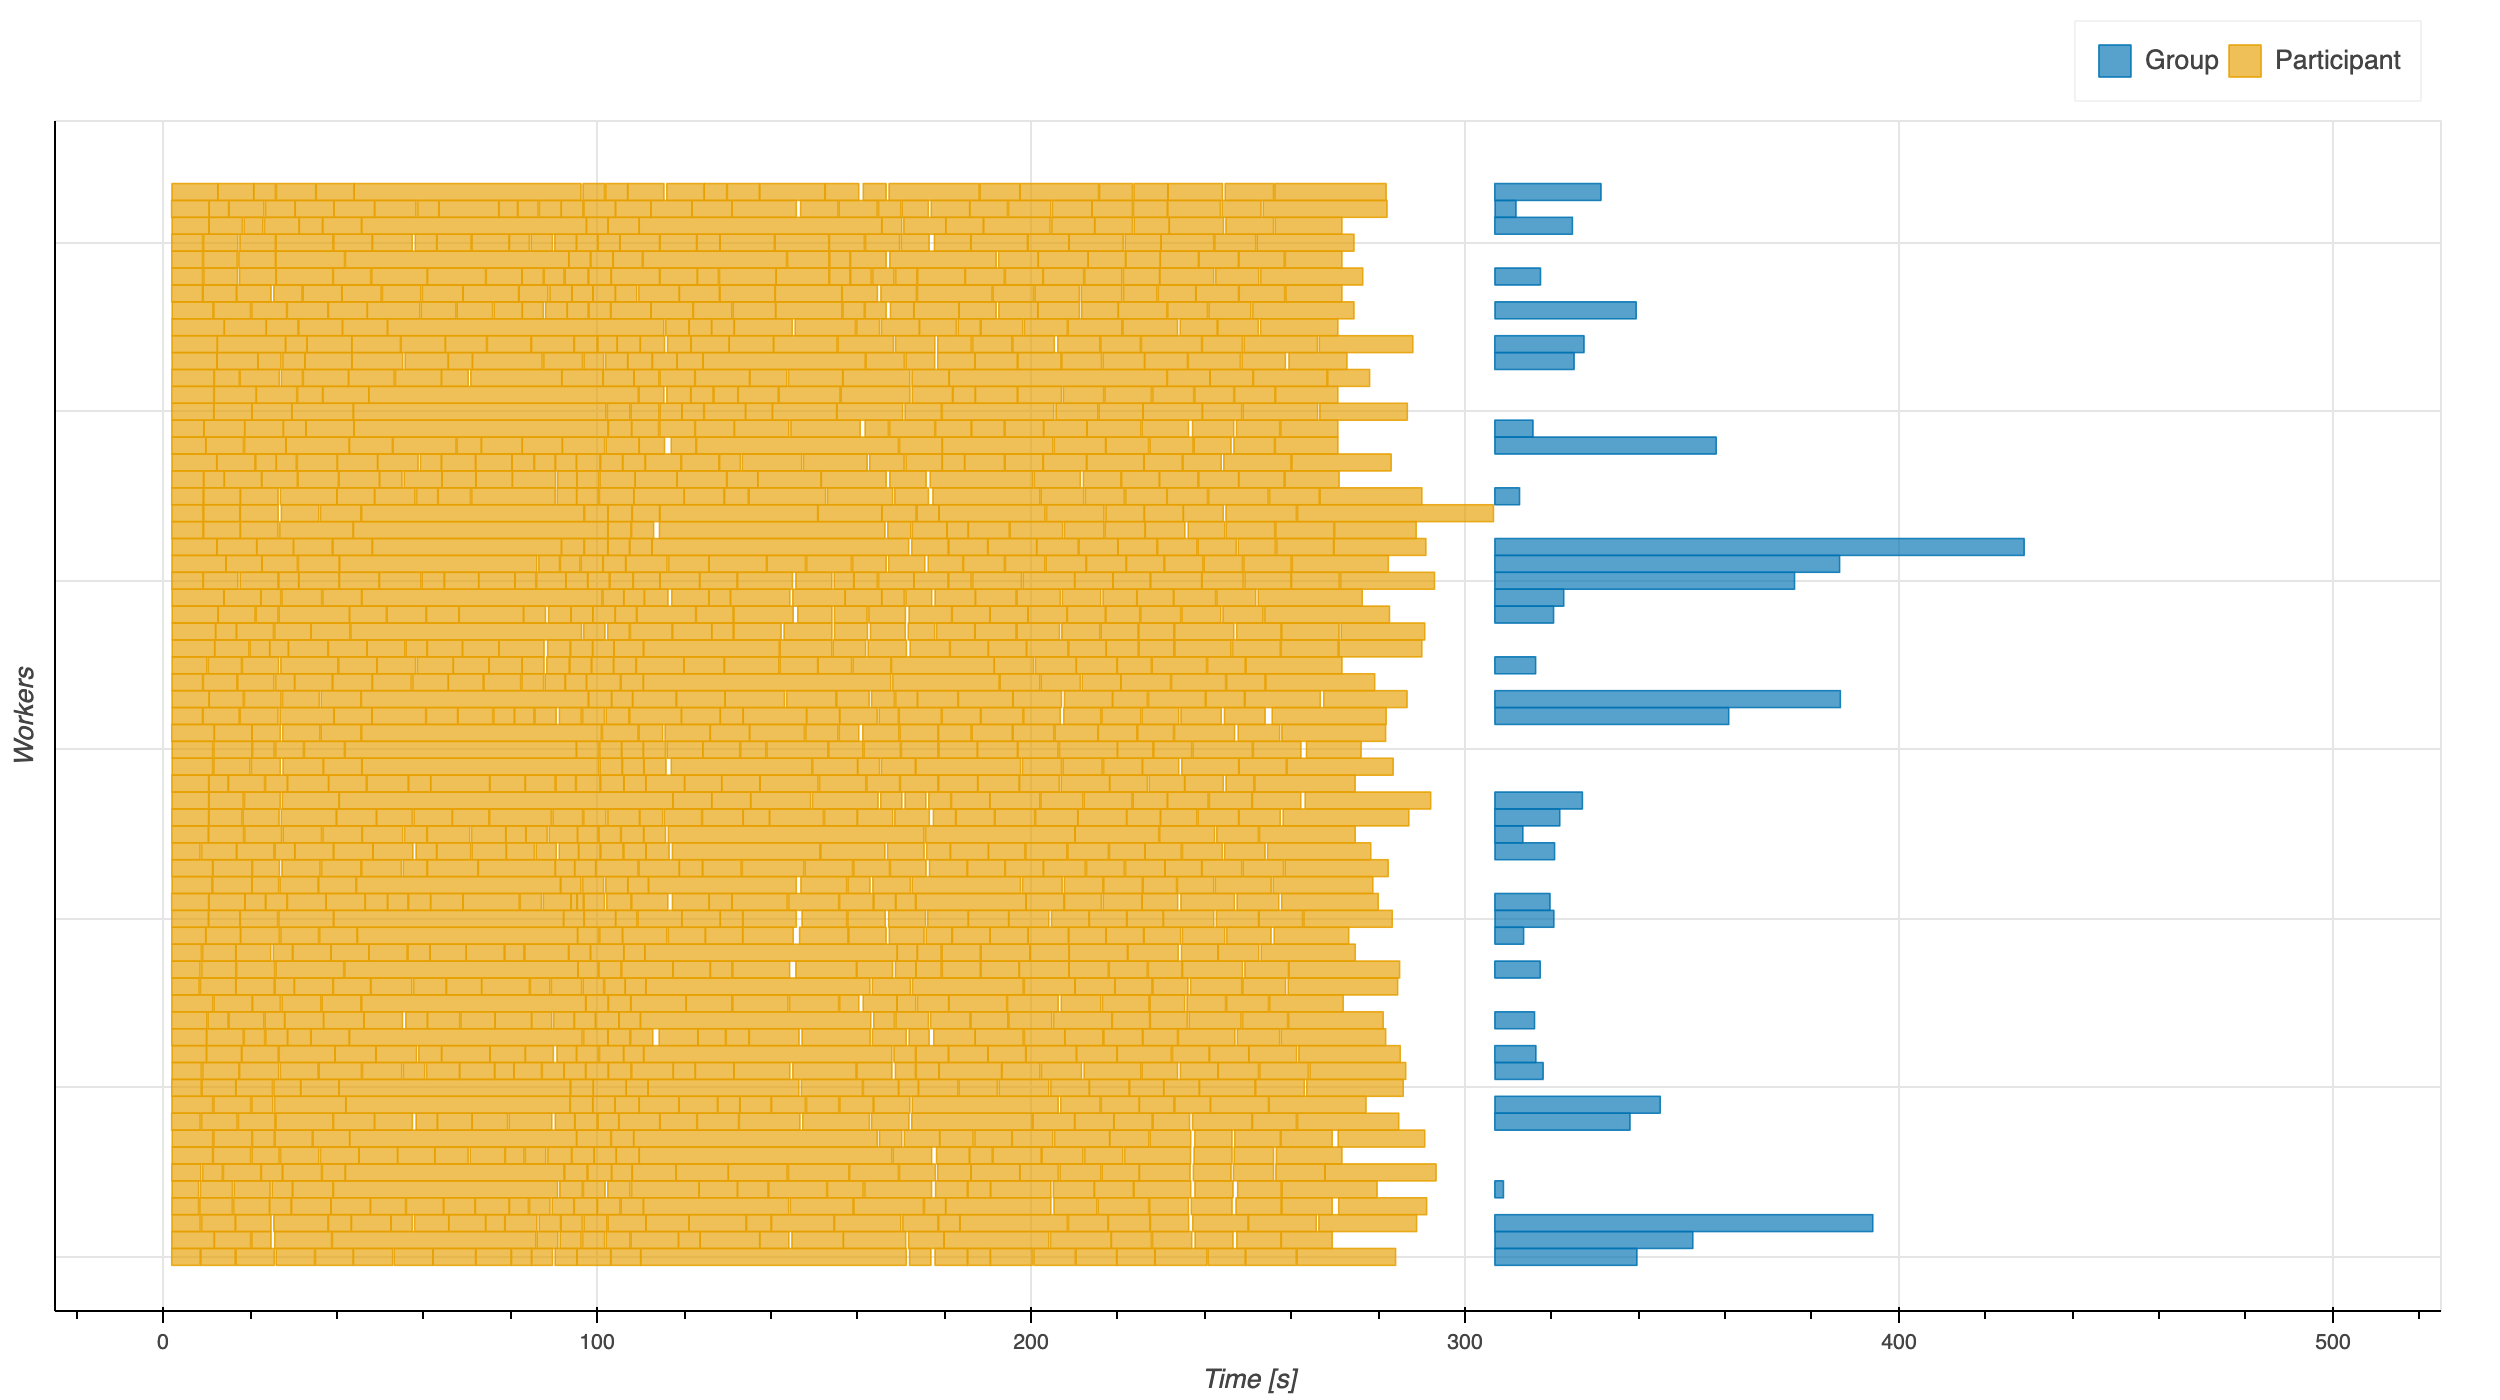
\includegraphics[clip,width=\columnwidth]{images/bag_bids_gantt.png}%
        \caption{Dask Bag}\label{fig:bids_dask_bag_gantt}
    \end{subfigure}
    \\
    \begin{subfigure}[b]{\columnwidth}
        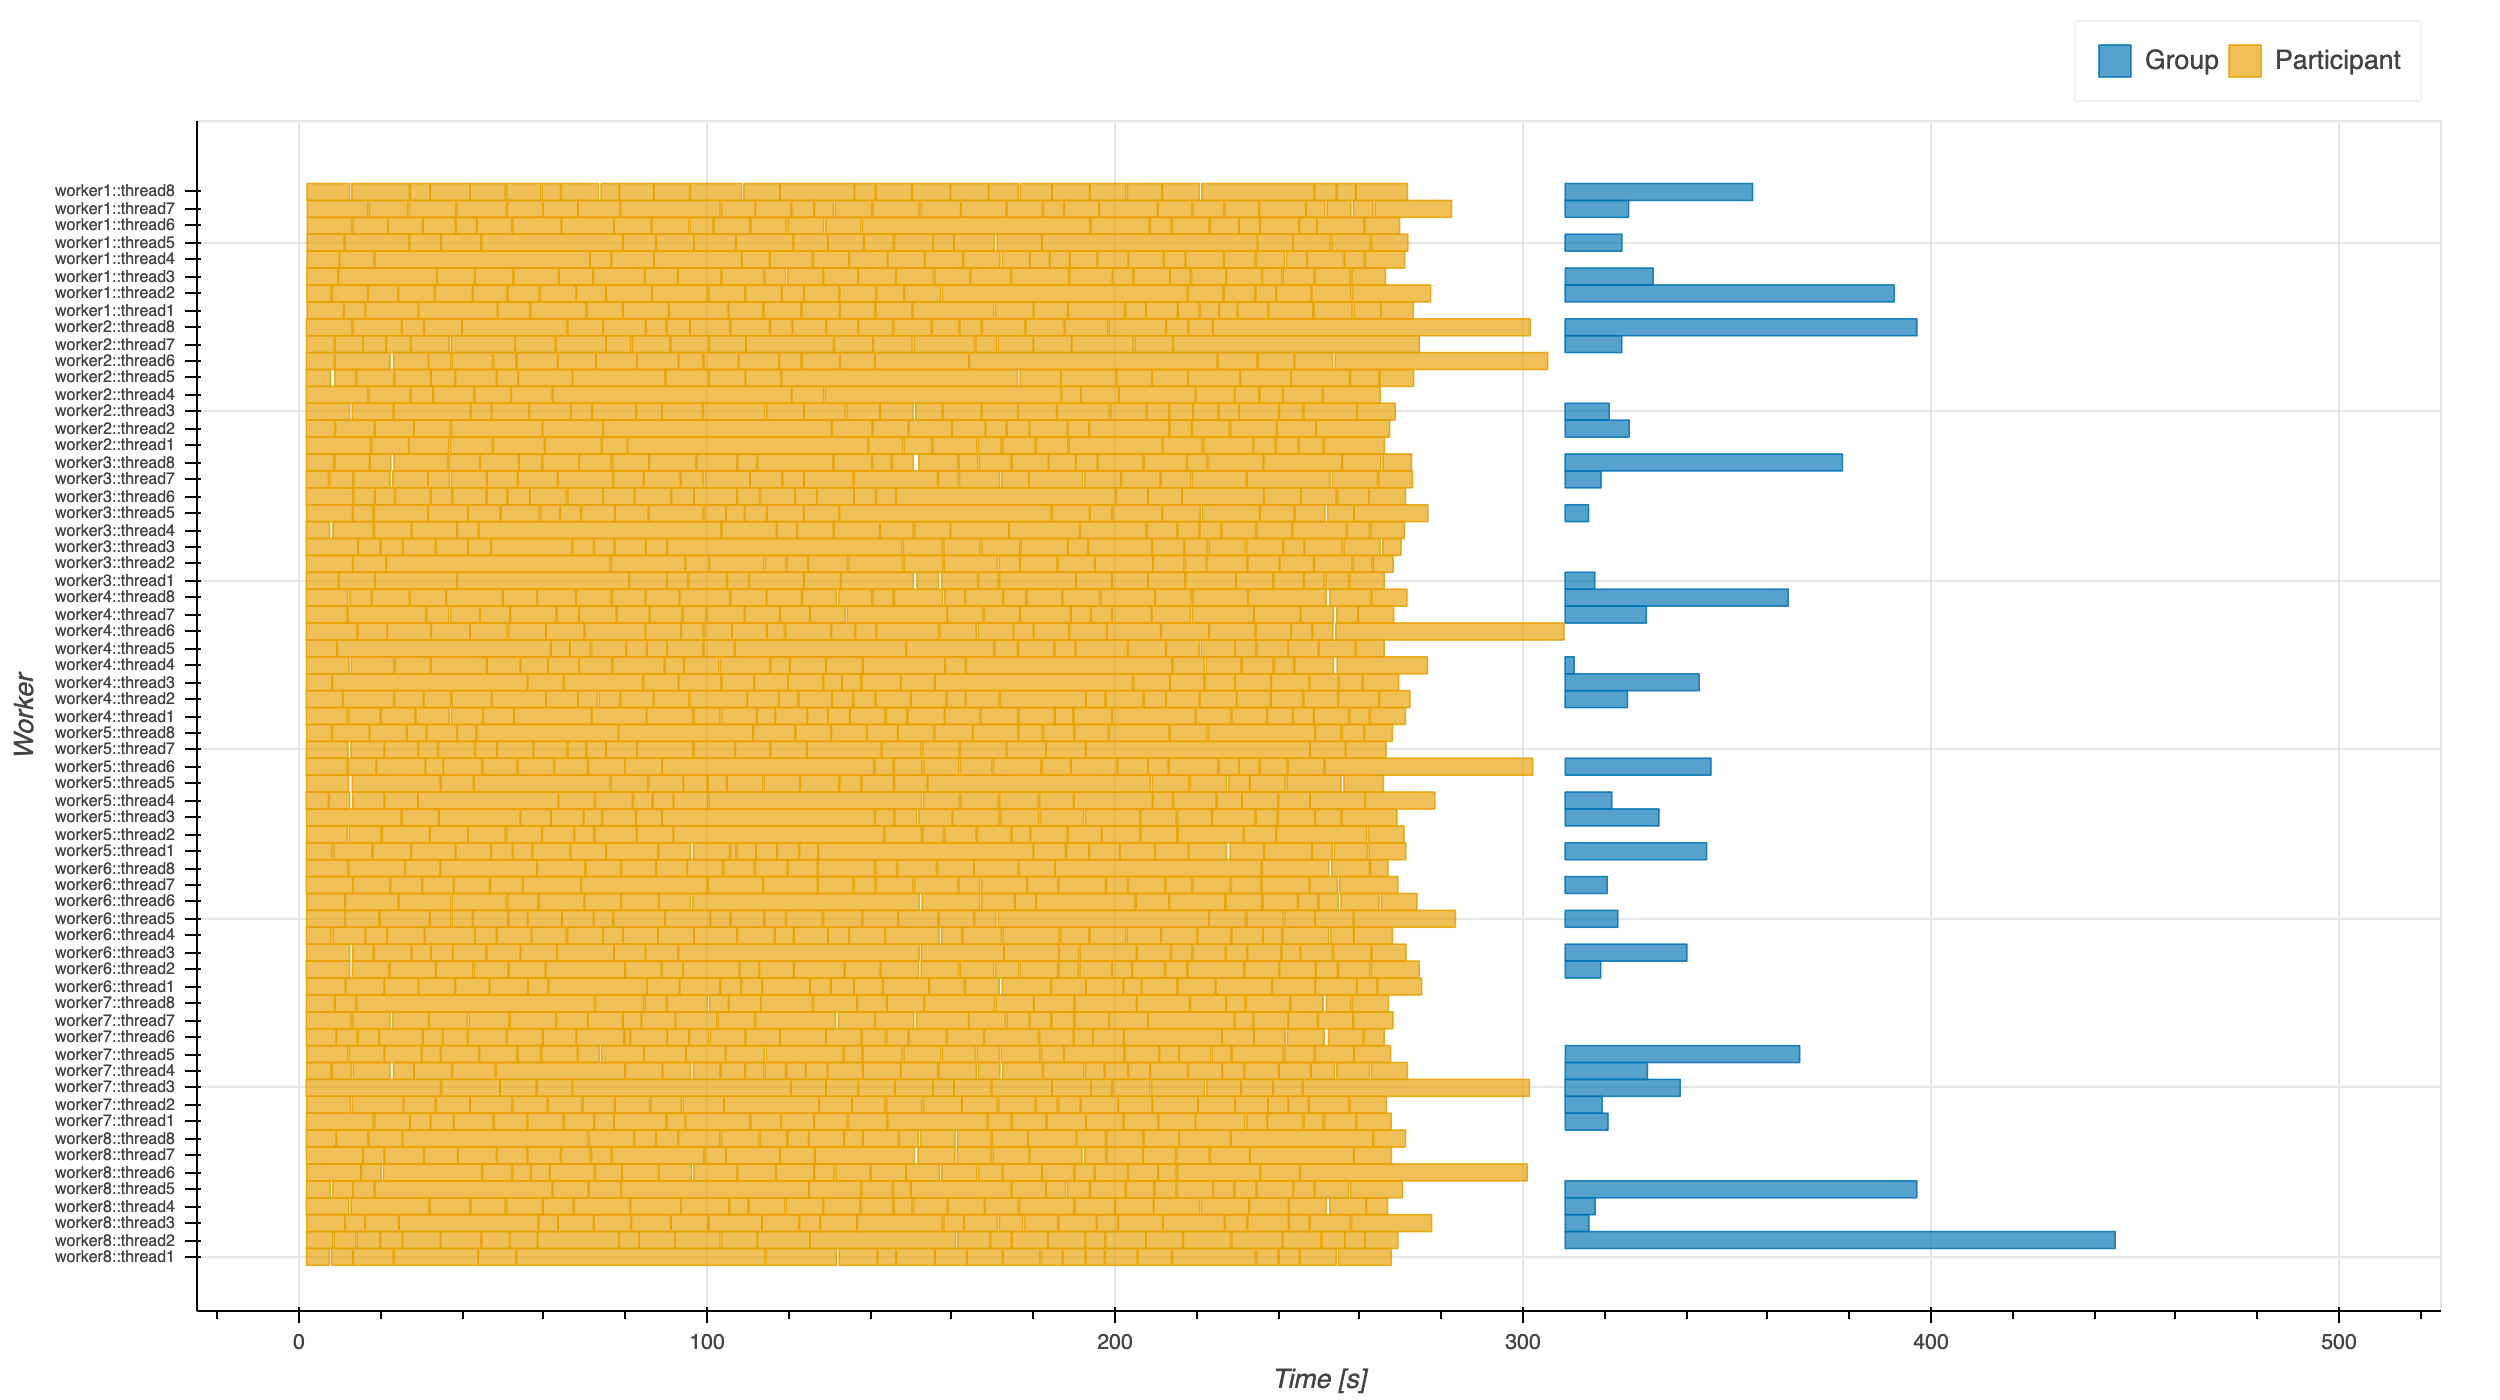
\includegraphics[clip,width=\columnwidth]{images/delayed_bids_gantt.png}%
        \caption{Dask Delayed}\label{fig:bids_dask_delayed_gantt}
    \end{subfigure}
    \hfill
    \begin{subfigure}[b]{\columnwidth}
        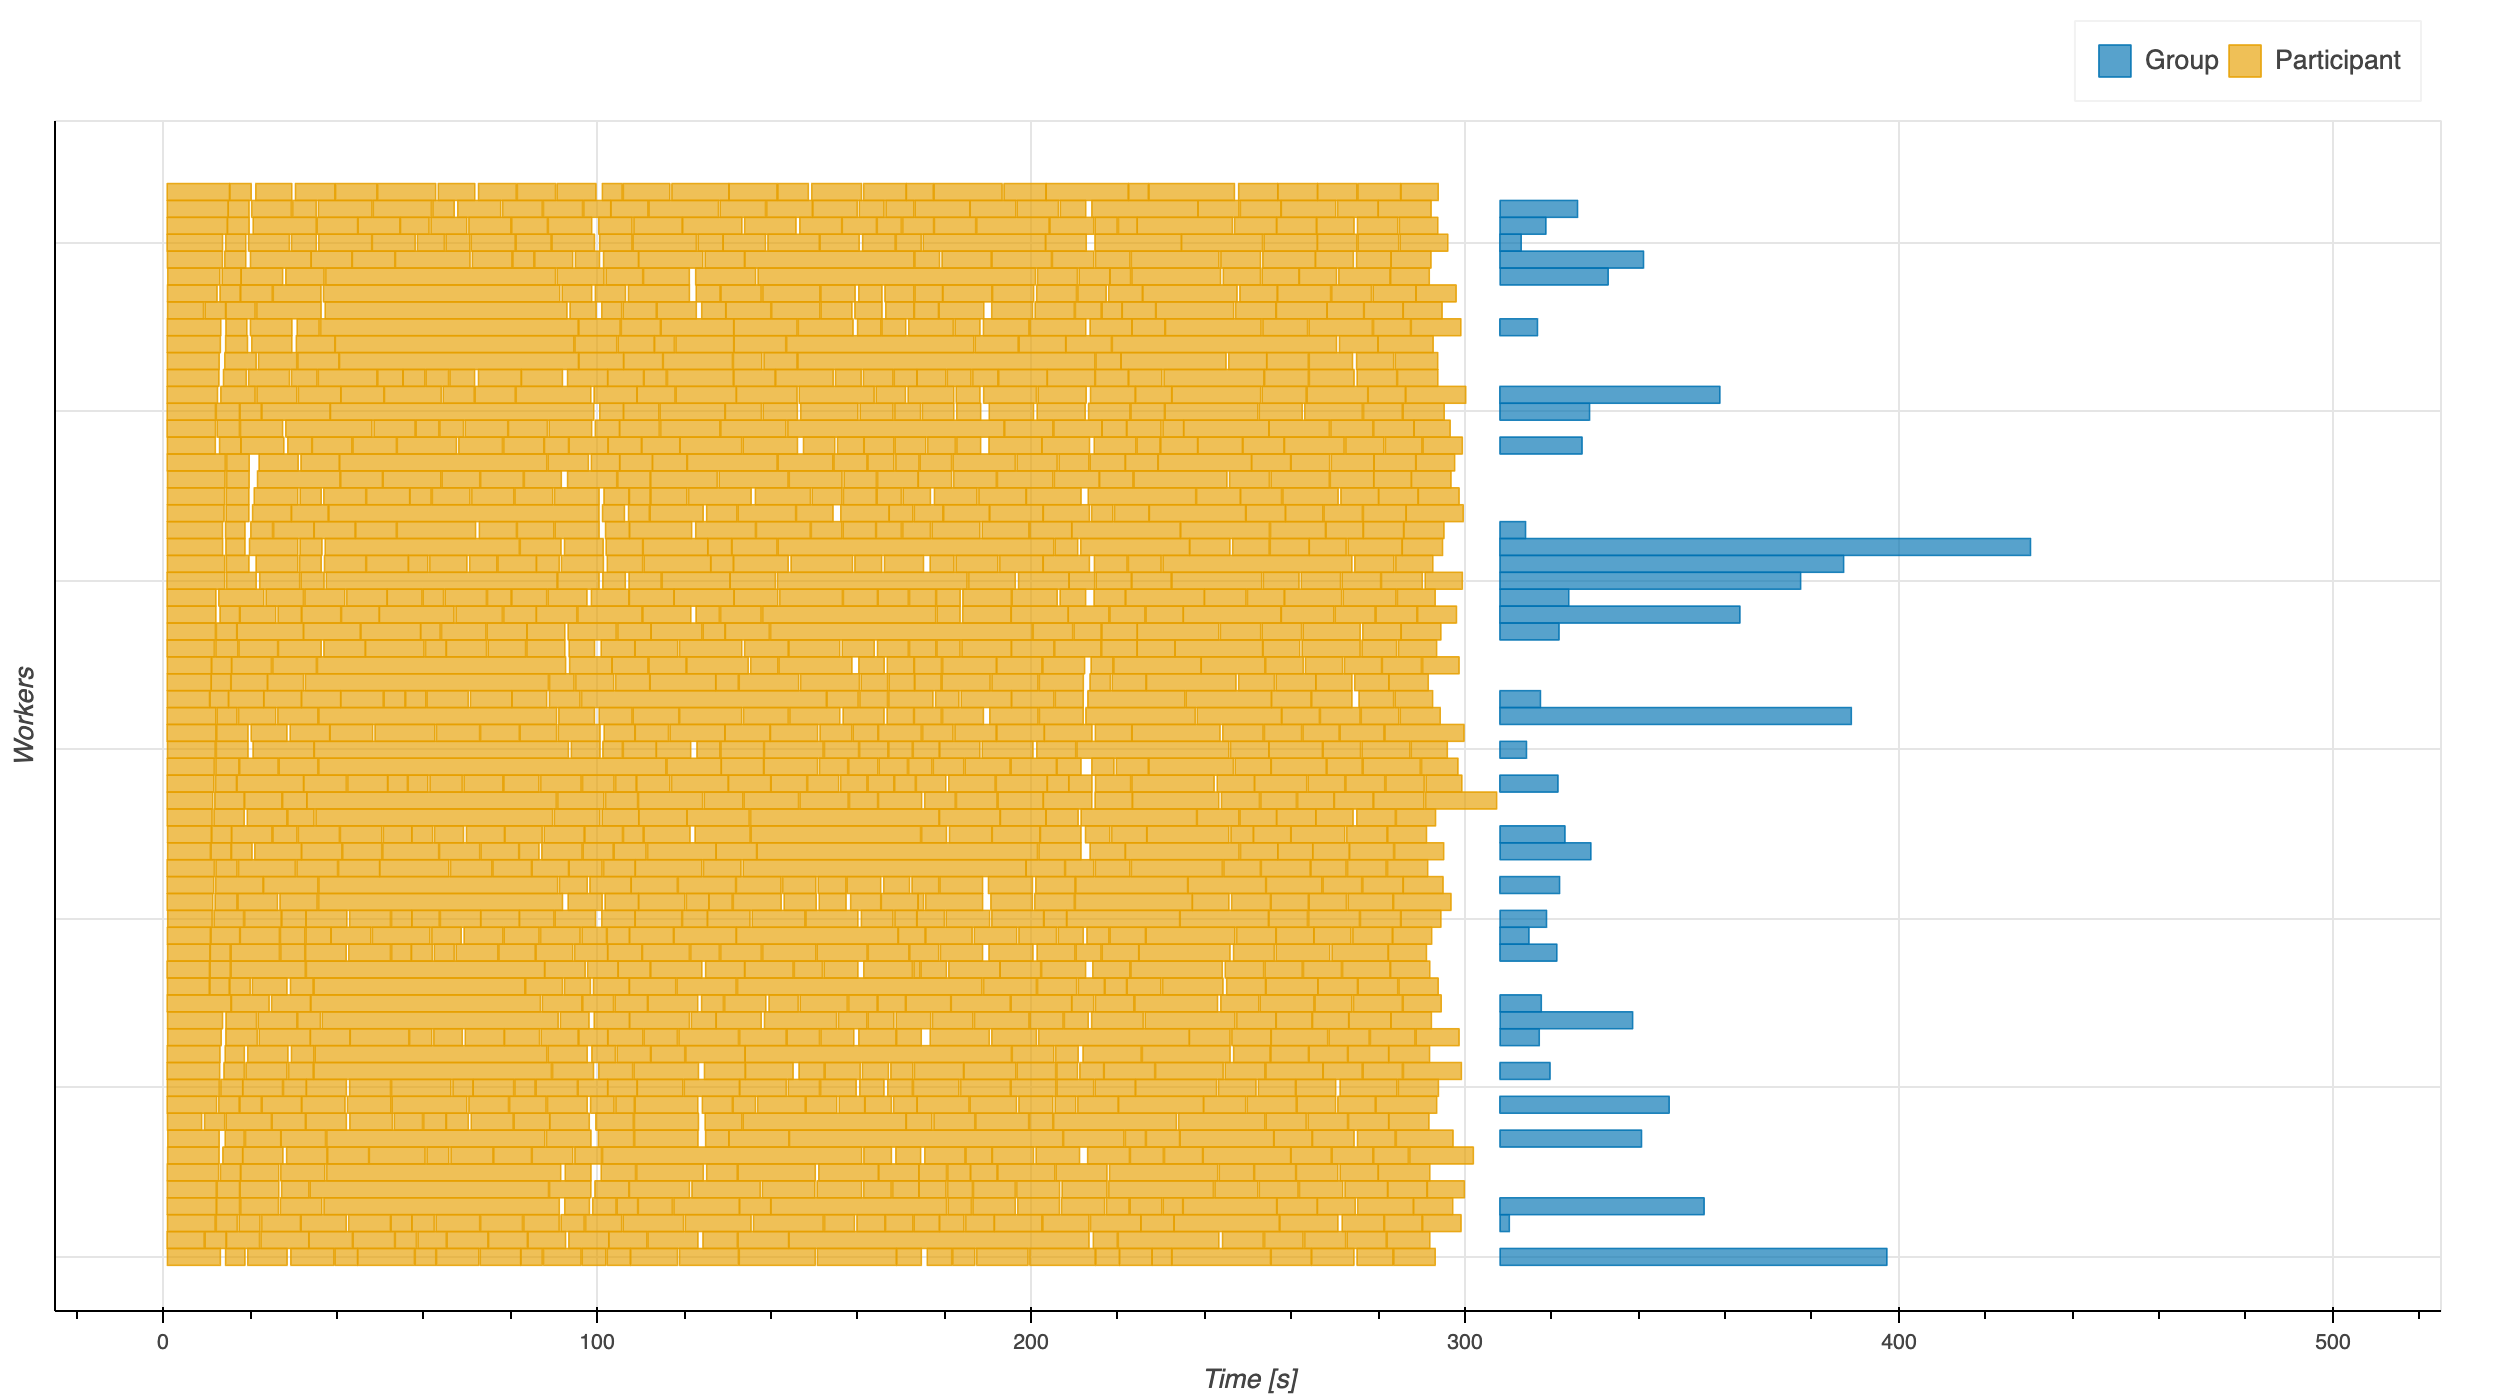
\includegraphics[clip,width=\columnwidth]{images/futures_bids_gantt.png}%
        \caption{Dask Futures}\label{fig:bids_dask_futures_gantt}
    \end{subfigure}
    \caption{Gantt chart with 8 workers}\label{fig:bids_gantt}
\end{figure*}



%%%%% DISCUSSION %%%%%
\section{Discussion}

\TG{Talk about engine overhead: (1) where is it coming from? (2) 
explain the impact on data transfers with a graph.}

\TG{In the dicussion, get back to it and mention that (1) we don't
always observe that, (2) for data-intensive applications, overheads don't really matter
as reducing them increases data trasnfers.}

% \subsection{IO Time}
% 
% 
% \subsection{Serialization}
% We think that serialization could have an important effect on the makespan of the
% application. This could potentially slow down the application when a lot of tasks are
% scheduled.
% 
% \subsection{NFS}
% The NFS seems to be a source of the bottleneck. We think that exploring another file
% system, like Lustre, could give us insight into the actual effect of the NFS on the
% application makespan. We also think that the NFS caching could play an effect on the
% task of different lengths.
% 
% \subsection{Scheduler}
% The Dask scheduler seems to have some bizarre behavior. It seems like it waits to
% schedule tasks. It could also be due to tasks being scheduled on other workers
% thus requiring data to be sent over the network; which would explain the stall on the
% worker. More work would be needed to investigate that issue.
% 
% 
% \subsection{Caching}
% We think that caching plays an effect on the results. As seen in the Gantt chart
% previously, some of the read tasks are significantly shorter than others while all
% blocks are of equal size.

\section*{Acknowledgment}

Mathieu Dugr\'e was funded by a Undergraduate Summer Research Assistant
award from the National Science and Engineering Research Council. We warmly
thank Compute Canada and \TG{Westgrid?} for providing the cloud
infrastructure used in these experiments, and the McGill Center for
Integrative Neurocience for giving us access to their cloud allocation.

\bibliographystyle{IEEEtran}
\bibliography{IEEEabrv,reference}

\end{document}
